\RequirePackage[l2tabu,orthodox]{nag}

% TODO: decide if one-sided/two-sided
%\documentclass[headsepline,footsepline,footinclude=false,fontsize=11pt,paper=a4,listof=totoc,bibliography=totoc,BCOR=12mm,DIV=12]{scrbook} % two-sided
\documentclass[headsepline,footsepline,footinclude=false,oneside,fontsize=11pt,paper=a4,listof=totoc,bibliography=totoc]{scrbook} % one-sided

% TODO: change citation style in settings
\PassOptionsToPackage{table,svgnames,dvipsnames}{xcolor}

\usepackage[utf8]{inputenc}
\usepackage[T1]{fontenc}
\usepackage[sc]{mathpazo}
\usepackage[ngerman,american]{babel}
\usepackage[autostyle]{csquotes}
\usepackage[%
  backend=biber,
  url=false,
  style=alphabetic,
  maxnames=4,
  minnames=3,
  maxbibnames=99,
  giveninits,
  uniquename=init]{biblatex} % TODO: adapt citation style
\usepackage{graphicx}
\usepackage{scrhack} % necessary for listings package
\usepackage{listings}
\usepackage{lstautogobble}
\usepackage{tikz}
\usepackage{pgfplots}
\usepackage{pgfplotstable}
\usepackage{booktabs}
\usepackage[final]{microtype}
\usepackage{caption}
\usepackage{enumitem}
\usepackage{amsmath}
\usepackage[hidelinks]{hyperref} % hidelinks removes colored boxes around references and links
\usepackage{caption}

\bibliography{bibliography}

\setkomafont{disposition}{\normalfont\bfseries} % use serif font for headings
\linespread{1.05} % adjust line spread for mathpazo font

% Add table of contents to PDF bookmarks
\BeforeTOCHead[toc]{{\cleardoublepage\pdfbookmark[0]{\contentsname}{toc}}}

% Define TUM corporate design colors
% Taken from http://portal.mytum.de/corporatedesign/index_print/vorlagen/index_farben
\definecolor{TUMBlue}{HTML}{0065BD}
\definecolor{TUMSecondaryBlue}{HTML}{005293}
\definecolor{TUMSecondaryBlue2}{HTML}{003359}
\definecolor{TUMBlack}{HTML}{000000}
\definecolor{TUMWhite}{HTML}{FFFFFF}
\definecolor{TUMDarkGray}{HTML}{333333}
\definecolor{TUMGray}{HTML}{808080}
\definecolor{TUMLightGray}{HTML}{CCCCC6}
\definecolor{TUMAccentGray}{HTML}{DAD7CB}
\definecolor{TUMAccentOrange}{HTML}{E37222}
\definecolor{TUMAccentGreen}{HTML}{A2AD00}
\definecolor{TUMAccentLightBlue}{HTML}{98C6EA}
\definecolor{TUMAccentBlue}{HTML}{64A0C8}

% Settings for pgfplots
\pgfplotsset{compat=newest}
\pgfplotsset{
  % For available color names, see http://www.latextemplates.com/svgnames-colors
  cycle list={TUMBlue\\TUMAccentOrange\\TUMAccentGreen\\TUMSecondaryBlue2\\TUMDarkGray\\},
}

% Settings for lstlistings
\lstset{%
  basicstyle=\ttfamily,
  columns=fullflexible,
  autogobble,
  keywordstyle=\bfseries\color{TUMBlue},
  stringstyle=\color{TUMAccentGreen}
}


% TODO: change thesis information
\newcommand*{\getUniversity}{Technische Universität München}
\newcommand*{\getFaculty}{Department of Informatics}
\newcommand*{\getTitle}{Annotation-efficient classification for biomedical images: combining active, self-supervised and semi-supervised}
\newcommand*{\getTitleGer}{Annotationseffiziente Klassifikation für biomedizinische Bilder: Kombination von aktiven, selbst-überwachten und semi-überwachten}
\newcommand*{\getAuthor}{Ahmad Bin Qasim}
\newcommand*{\getDoctype}{Master's Thesis}
\newcommand*{\getSupervisor}{Prof. Dr. Bjoern Menze}
\newcommand*{\getAdvisor}{Dr. Carsten Marr, Ali Boushehri, Dominik Waibel, Ivan Ezhov}
\newcommand*{\getSubmissionDate}{15.12.2020}
\newcommand*{\getSubmissionLocation}{Munich}

\begin{document}

% Set page numbering to avoid "destination with the same identifier has been already used" warning for cover page.
% (see https://en.wikibooks.org/wiki/LaTeX/Hyperlinks#Problems_with_Links_and_Pages).
\pagenumbering{alph}
\begin{titlepage}
  % HACK for two-sided documents: ignore binding correction for cover page.
  % Adapted from Markus Kohm's KOMA-Script titlepage=firstiscover handling.
  % See http://mirrors.ctan.org/macros/latex/contrib/koma-script/scrkernel-title.dtx,
  % \maketitle macro.
  \oddsidemargin=\evensidemargin\relax
  \textwidth=\dimexpr\paperwidth-2\evensidemargin-2in\relax
  \hsize=\textwidth\relax

  \centering

  \IfFileExists{logos/tum.pdf}{%
    
\includegraphics[height=20mm]{logos/tum.pdf}
  }{%
    \vspace*{20mm}
  }

  \vspace{5mm}
  {\huge\MakeUppercase{\getFaculty{}}}\\

  \vspace{5mm}
  {\large\MakeUppercase{\getUniversity{}}}\\

  \vspace{20mm}
  {\Large \getDoctype{}}

  \vspace{15mm}
  {\huge\bfseries \getTitle{}}

  \vspace{15mm}
  {\LARGE \getAuthor{}}

  \IfFileExists{logos/faculty.pdf}{%
    \vfill{}
    \includegraphics[height=20mm]{logos/faculty.pdf}
  }{}
\end{titlepage}


\frontmatter{}

\begin{titlepage}
  \centering

  \IfFileExists{logos/tum.pdf}{%
    
\includegraphics[height=20mm]{logos/tum.pdf}
  }{%
    \vspace*{20mm}
  }

  \vspace{5mm}
  {\huge\MakeUppercase{\getFaculty{}}}\\

  \vspace{5mm}
  {\large\MakeUppercase{\getUniversity{}}}\\

  \vspace{20mm}
  {\Large \getDoctype{}}

  \vspace{15mm}
  {\huge\bfseries \getTitle{} \par}

  \vspace{10mm}
  {\huge\bfseries \foreignlanguage{ngerman}{\getTitleGer{}} \par}

  \vspace{15mm}
  \begin{tabular}{l l}
    Author:          & \getAuthor{} \\
    Supervisor:      & \getSupervisor{} \\
    Advisor:         & \getAdvisor{} \\
    Submission Date: & \getSubmissionDate{} \\
  \end{tabular}

  \IfFileExists{logos/faculty.pdf}{%
    \vfill{}
    \includegraphics[height=20mm]{logos/faculty.pdf}
  }{}
\end{titlepage}

\thispagestyle{empty}
\vspace*{0.8\textheight}
\noindent
I confirm that this \MakeLowercase{\getDoctype{}} is my own work and I have documented all sources and material used.

\vspace{15mm}
\noindent
\getSubmissionLocation{}, \getSubmissionDate{} \hspace{50mm} \getAuthor{}

\cleardoublepage{}

\chapter{\abstractname}

%TODO: Abstract




\microtypesetup{protrusion=false}
\tableofcontents{}
\microtypesetup{protrusion=true}

\newpage

\addcontentsline{toc}{chapter}{Abbreviations}
\thispagestyle{empty}

{\usekomafont{section} Abbreviations}

\vspace{10mm}

AML = Acute myeloid leukemia

ANNs = Artificial Neural Networks

CNNs = Convolutional Neural Networks

FN = False Negative

FP = False Positive

ISIC = International Skin Imaging Collaboration

MC-Dropout = Monte Carlo Dropout

MLP = Multi-Layer Perceptron

ReLU = Rectified Linear Unit

SGD = Stochastic Gradient Descent

SimCLR =  A Simple Framework for Contrastive Learning of Visual Representations

SSL = Semi-supervised Learning

TL = Transfer learning

TN = True Negative

TP = True Positive

\cleardoublepage{}

\addcontentsline{toc}{chapter}{Acknowledgments}
\thispagestyle{empty}


{\usekomafont{section} Acknowledgments}

\vspace{10mm}

First, I want to thank my external supervisor Dr. Carsten Marr, at Institute of Computational Biology, Helmholtz Center, Munich. I am thankful to him for creating a productive working environment and for providing his valuable feedback throughout the course of my thesis. I also want to thank my advisors Ali Boushehri and Dominik Waibel. They supported me greatly by providing guidance during our weekly meetings and discussions. They also took the lead with writing a research paper based on the findings of the thesis. We submitted the research paper to Conference on Computer Vision and Pattern Recognition (CVPR) 2021. I also want to thank my supervisor Prof. Dr. Bjoern Menze from the TUM for supervising my master thesis. \\
I want to thank my friends and family, who rendered their full support during the course of the thesis.

\cleardoublepage{}


\mainmatter{}

% !TeX root = ../main.tex
% Add the above to each chapter to make compiling the PDF easier in some editors.

\chapter{Introduction}\label{chapter:introduction}

\section{Machine Learning}
Machine learning is the process which enables computer programs to perform tasks without hard-coding the solution programmatically by learning from data provided to them. Computers can be explicitly programmed to perform simple tasks such as arithmetic operations but for advanced tasks, it comes progressively more difficult to program computers explicitly. In this case, it becomes more feasible to let a computer learn the steps which it needs to perform for performing a certain advanced task. \\
Machine learning deploys various approaches which allow the computers to learn to perform advanced tasks by finding out a suitable algorithm on its own without programming all of the steps needed to find a solution to the tasks. A subset of machine learning approaches, depend upon help in the form of annotated data i.e. to label the data so that the computer can find better solutions to the tasks in light of the information added through the labels. \\
Machine Learning approaches can be categorized into four categories:
\begin{itemize}
  \setlength\itemsep{0em}
  \item Supervised learning: The computer is provided data which contains examples and their respective desired outputs, by an "oracle", and the computer aims to learn a generalized mapping from the examples to the respective outputs.
  \item Unsupervised learning: The computer is provided data without specifying the desired outputs for the examples. The computer is expected to learn the inherent structure of the data based on the examples.
  \item Semi-supervised learning: The computer tries to learn a mapping from the inputs to outputs with help from data with labels as well as the data without labels. Semi-supervised learning can be the other way around too, where the computer learns the inherent structure of data with the help of labeled examples in addition to examples without any labels.
  \item Reinforcement learning: The computer interacts with an environment which is often simulated. It tries to fulfill a goal by performing different actions within the environment. The environment provides feedback to the computer which allows the computer to learn the right actions.
\end{itemize}
Recently, deep learning has become more popular in machine learning circles.

\section{Artificial neural networks}
Artificial neural networks (ANNs) also known as connectionist systems are inspired by biological organisms. The biological brains consist of millions or billions of neurons connected together in the form of a network. ANNs learn specific tasks without being programmed explicitly with rules. \\
An ANN is based on "artificial neurons", which are connected together in the form of a network which is inspired by biological networks of neurons in animal brains. In animal brains, the signals travel through neural pathways in the form of electric pulses and each neuron can signal other connected neurons to activate if the electric pulse is above a certain threshold. An "artificial neuron" in the same way can activate other neurons connected to it. \\
Typically the ANNs are implemented such that the signals at the neurons are real numbers and the outputs are calculated by defining a non-linear function on the sum of the inputs to the ANNs. The connecting pathways between the ANNs are given some weights which are adjusted as the training process continues. The weights of the connections are increased or decreased depending upon the value of the input signals. ANNs are typically organized into layers. The output of each preceding layer is added as an input of the next layer. Each layer manipulates the input in a different way. The output of the last layer is used as the final prediction. \\
The goal of ANNs was to simulate a animal brain neural network but with time the focus shifted towards more specific tasks. Nowadays, ANNs are being for computer vision and natural language processing etc. \\
Deep learning involves several hidden layers stacked together in an ANN. Applications of deep learning include computer vision and natural language processing.

\section{Deep Learning}
Deep learning models are typically based on ANNs. Convolutional Neural Networks (CNNs) are the most commonly used ANNs for deep learning. In deep learning several hidden layers of ANNs are stacked together. \\
In deep learning, each layer learns a different transformation of the inputs, which tend to be more abstract as the network gets deeper. For example, in case of an image of a car, in order to detect the image as a car, the first layer may learn the structure of pixels and the edges, the second layer may learn the arrangement of edges, the third layer may learn specific areas of the image such as wheels or steering, the fourth layer may learn the overall shape of the car. The main allure of deep learning models is that, the model can learn to place the features in different layers without any help. "Deep" refers to the number of layers of ANNs in a deep learning model.

\section{Active learning}
Active learning\cite{settles2009} tries to mitigate the cost of annotating the datasets, by efficiently selecting the data points, which can be annotated for maximum performance gain on the underlying task. \\
Active learning is a subfield of machine learning. The main idea behind active learning is that, the active learning algorithm chooses the data that the model should learn from. This is an important characteristic, because deep learning models can require thousands of labeled examples to achieve good performance. More annotated data results in superior performance. Sometimes, the cost of obtaining annotations is not high, e.g. the data obtained from users on social media or the data gathered by websites in a passive way about user behaviour, but obtaining annotations can be very costly and time-consuming. The cost of annotations varies depending upon the underlying deep learning task. Compared to classification tasks, segmentation tasks have significantly higher costs as the annotation process has to be carried out on the pixel-level. Similarly, object detection requires labor and time intensive bounding boxes to be drawn over the target images. The cost of annotation gets even high in the biomedical domain. Due to the safety critical nature of medical data, multiple experts have to be consulted for annotating biomedical datasets. \\
Hence, active learning algorithms try to achieve good performance while using as less data points as possible. They do so, by selecting the data points as shown in figure \ref{fig:active_learning}, which can have the most positive effect on the model's performance. As a result, active learning algorithms reduce the overall cost of data annotation.

\begin{figure}[htbp]
\centering
\captionsetup{format=plain}
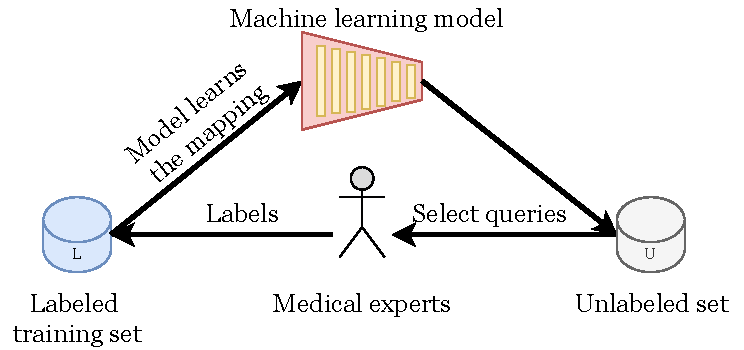
\includegraphics[width=0.75\textwidth]{figures/fig_active_learning.pdf}
\caption{The labeled set $\mathcal{L}$ is used to train the model. The trained model is then used to select data points, through an active learning algorithm, from the unlabeled set $\mathcal{U}$ for annotation. The selected data points are annotated by an expert and added to the labeled set $\mathcal{L}$.}
\label{fig:active_learning}
\end{figure}

% make this bigger and take help from https://link.springer.com/article/10.1007/s10994-019-05855-6
\section{Semi-supervised learning}
Semi-supervised learning (SSL)\cite{van2020} mitigates the requirement for labeled data by providing a means of leveraging unlabeled data. \\ Semi-supervised learning is a subfield of machine learning which tries to combine supervised learning with unsupervised learning. Semi-supervised learning algorithms, try to use the information available in the unlabeled data domain to help the performance of the model in the labeled data domain or vice versa. For instance, in case of a classification task, the data points without a label can be help with the classification task. For an unsupervised method such as clustering, it can be helpful to have some data points which are known to belong to a specific class. \\
There are many cases where unlabelled data can help in constructing a classifier. Consider the example of a regression model, where the model takes images of a house as input and it has to predict the price of a house. Suppose the model learns to predict a higher price for houses with a parking space compared to the houses which don't have this predictive property. This regression model might work well for the examples in the training set that contain the predictive property of having a parking space, but will fail when the input images do not contain that predictive property. For example, if a house doesn't have a parking space but it has other amenities such as a swimming pool, the model will still predict a lower price for that house. Semi-supervised learning can be helpful in this regard. Consider that the unlabeled dataset, might contain some data points which connect the predictive property of having a parking space to the property of containing a swimming pool. For instance, the property of having a parking space might co-occur with the property of having a balcony. Moreover, the property of having a balcony might co-occur with the property of having a swimming pool. Hence, the model might be able to predict a higher price for a house containing a swimming pool, even if it has not seen that property in the training set.\\
SSL operates on the assumption that the unlabeled data contains some prior information about the labeled data. Since unlabeled data can often be obtained with minimal human labor, any performance boost conferred by SSL often comes with low cost. \\

\begin{figure}[htbp]
\centering
\captionsetup{format=plain}
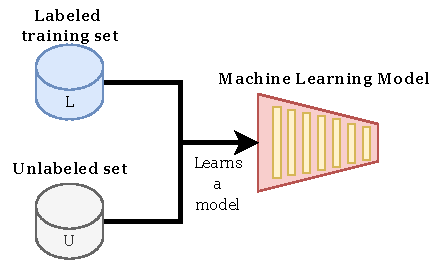
\includegraphics[width=0.5\textwidth]{figures/fig_semi_supervised_learning.pdf}
\caption{In SSL, both, the labeled set $\mathcal{L}$ and the unlabeled set $\mathcal{U}$, are used for learning a model. The information in the unlabeled set $\mathcal{U}$ is harnessed to improve the training performance on labeled set $\mathcal{L}$.}
\label{fig:semi_supervised_learning}
\end{figure}

\section{Annotation-efficient deep learning}
Deep learning methods are dependent upon large amounts of annotated data for their success \cite{sun2017}. In case of biomedical images, the annotations have to carried out by trained experts, so the process of annotations is time-consuming and expensive. Active learning algorithms try to minimize the need of annotations by selecting the data points which are most informative for annotation \cite{settles2009, sadafi2019, joshi2009}, but these algorithms are usually tested on real world image datasets e.g. ImageNet \cite{gal2016, ducoffe2015, holub2008}. However, biomedical images do not posses the same properties as real world images. Biomedical images have little variation between classes and posses little difference in color and textures \cite{matek2019, esteva2017}. Furthermore, biomedical image datasets have high class imbalance, which can have an significant impact on the results e.g. an algorithm which performs quite good for a dataset with no class imbalance might not perform as well for a dataset with high class imbalance. It has been shown that active learning can work well for biomedical image classification \cite{sadafi2019, smailagic2018} and segmentation \cite{yang2017}. However it is not clear that which active learning algorithm is more suited for a particular kind of biomedical image data and how can the active learning algorithms be combined with other deep learning methods for improving their performance. \\
It has been shown that pre-training methods such as transfer learning and self-supervised learning show great promise for initialization of network weights when low amount of annotation data is available \cite{chen2020, oord2018, newell2020, sagheer2019}. For transfer learning, the network weights are learned by training on a similar dataset and then reusing the learned weights for network initialization while training on the target dataset \cite{jing2020}. Initialization using pre-trained ImageNet weights is the most common transfer learning method and has been used in many biomedical applications for network initialization \cite{rajpurkar2017, wang2017}. However it is shown by Raghu and Zhang et al. \cite{raghu2019} that in transfer learning using ImageNet weights does not lead to an improvement in the performance for many biomedical image datasets. Moreover, it is shown that self-supervised learning on biomedical images can lead to an increase in performance \cite{holmberg2020}. \\
Finally, semi-supervised learning has been shown to increase the performance and stability of results \cite{sohn2020, tarvainen2017}. High-throughput methods are regularly employed in biomedical imaging \cite{blasi2016} to obtain a large number of unlabeled data points. However, as mentioned earlier, annotations are scarce in the domain of biomedical imaging. Thus, semi-supervised methods have great potential in this domain. \\
In this thesis, firstly, a comparison has been made between different active learning methods. Secondly, the performance of the active learning algorithm which performed the best, is further improved by adding pre-training and semi-supervised learning. To find out if a certain combination of the three active learning algorithms in addition to random sampling (baseline), three pre-training methods plus random initialization (baseline) and two training strategies which include supervised and semi-supervised learning, can outperform other conventional methods, an extensive grid search is performed and the results are gathered on three biomedical image datasets. As a result, an optimal strategy is found.
% !TeX root = ../main.tex
% Add the above to each chapter to make compiling the PDF easier in some editors.

\chapter{Datasets}\label{chapter:datasets}
This thesis shows the performance of different active learning algorithms, pre-training methods and training strategies on three biomedical image datasets, as shown in Figure \ref{fig:datasets_composition}.

\begin{figure}[htbp]
\centering
\captionsetup{format=plain}
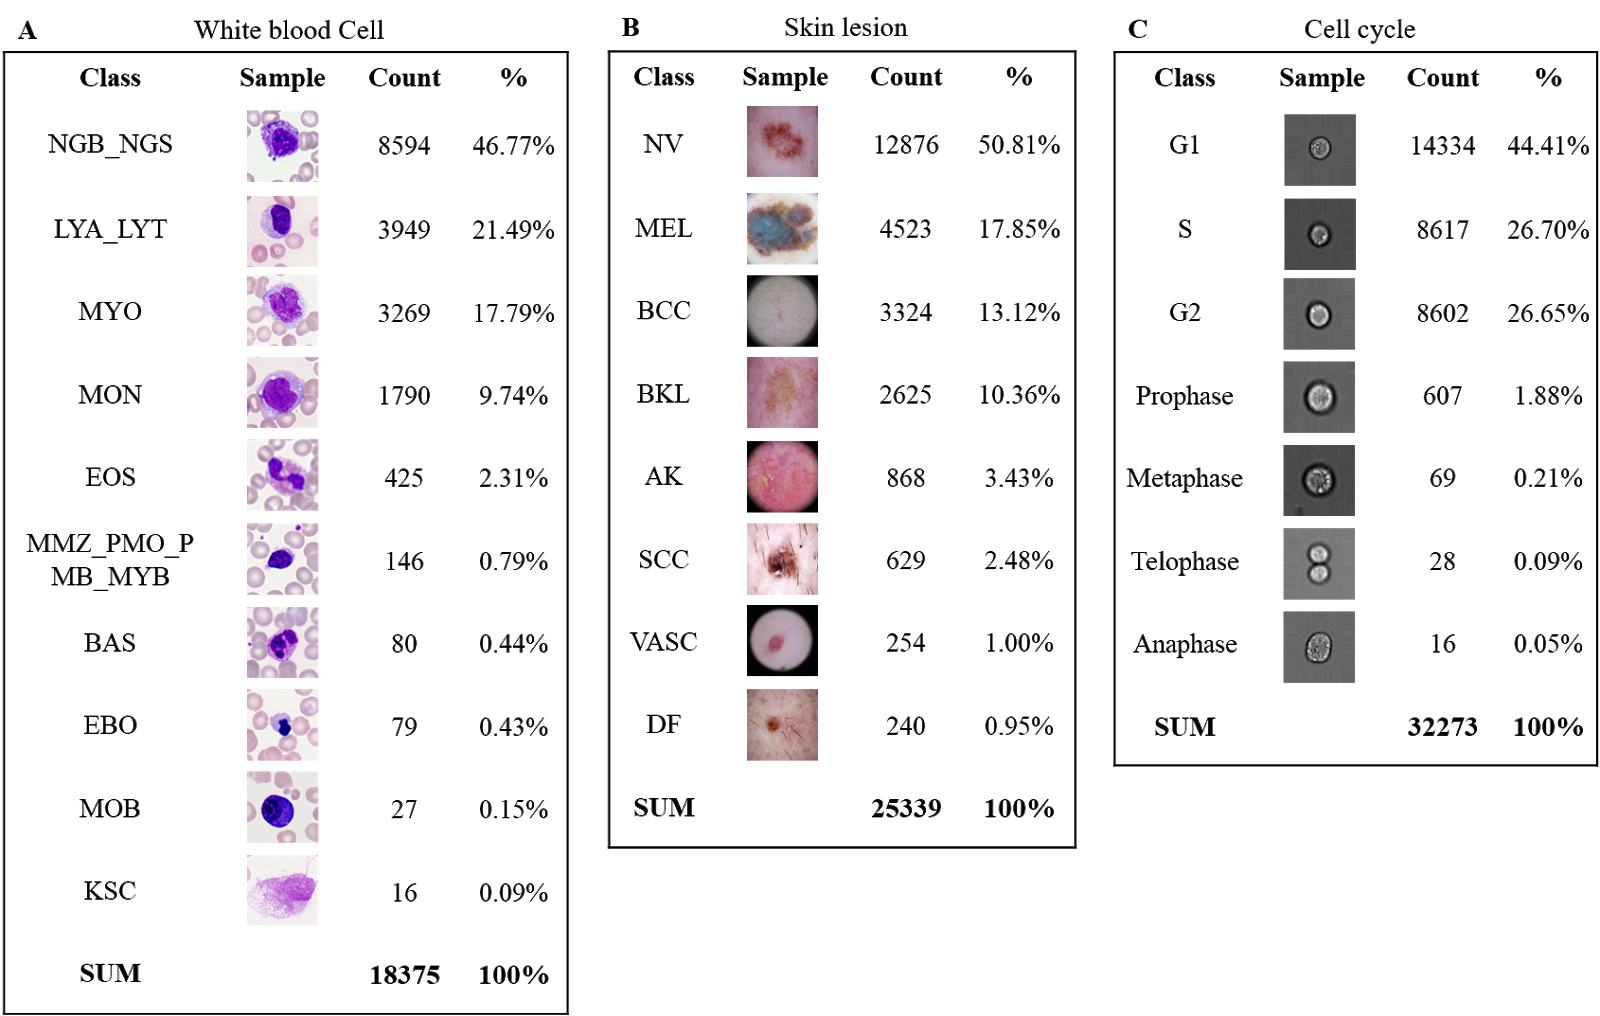
\includegraphics[width=0.95\textwidth]{figures/fig_datasets_composition.png}
\caption{The biomedical image datasets shown in this thesis have high class imbalance, low levels of contrast between different colors and a high level of similarity between different classes (A) White blood cell: This dataset contains 18357 (128x128) single-cell images. They are taken from peripheral blood smears of 100 patients diagnosed with AML, as well as 100 patients without any symptoms of the disease. \cite{matek2019, clark2013}. (B) Skin lesion: This dataset contains 25339 (128x128) images obtained using Dermoscopy. The images are classified into eight classes which specify different skin cancer types. \cite{codella2018, combalia2019, tschandl2018}. (C) Cell cycle: A dataset comprising 32272 images (64x64 pixel) of Jurkat cells in seven different cell cycle stages created by imaging flow cytometry \cite{eulenberg2017}.}
\label{fig:datasets_composition}
\end{figure}

\newpage

% rework these sections to make them different from what it says on their websites
\section{White Blood Cells}

The White Blood Cells Dataset contains 18357 single-cell images labeled by experts taken from peripheral blood smears of 100 patients diagnosed with AML, as well as 100 patients without any symptoms of the disease. 

White blood cells, also known as leukocytes or leucocytes, are the cells which protect the body from foreign objects and infections. White blood cells are found throughout the body including the blood.

AML is a cancer occurring in the myeloid line of blood cells. Its symptoms include the rapid growth of abnormal cells which interfere with normal blood cells production due to a build-up in the bone marrow and the blood. Symptoms can include continuous feeling of tiredness, being out of breath frequently, and high risk of infection. At certain occasions, the cancer can metastasize and spread to other organs of the body. AML progresses quickly and can prove to be fatal in a matter of months. AML is initially treated using chemotherapy. The goal of chemotherapy is to set a remission in motion. Other treatments include radiation therapy or a stem cell transplant. The treatment is guided by the type of mutation present within the body. This also dictates, how long a person is likely to live.

During the formulation of the dataset, the malignant and non-malignant white blood cells were classified into a standard morphological classification scheme. To quantify account of uncertainties between the expert labeling, a subset of images was re-annotated up to two times.

The dataset has been used as the primary dataset for testing different active learning algorithms, training strategies and pre-training methods.

\section{Skin Lesion}

The Skin Lesion dataset is developed by The International Skin Imaging Collaboration (ISIC): Melanoma project. The goal of the melanoma project is the application of medical imaging using computational technologies for detection of melanoma and eventually the reduction of melanoma mortality.

Melanoma, also called malignant melanoma, is a type of skin cancer. It is developed within the melanocytes cells. Melanocytes are responsible for producing pigments in the skin. Melanomas can also occur in other organs such as the mouth, intestines and the eye. About 25\% of melanomas develop from moles. Symptoms such as increase in the size of a mole, irregular edges, color changes, itchiness or skin breakdown can indicate melanoma.

Melanoma treatment heavily depends on early detection. If detected in its early stages, Melanoma is readily curable. Skin lesion imaging can not only help with the education of experts and the public but it can also be used for automated diagnosis, decision support in clinics and teledermatology. The quality of skin lesion imaging is hampered by a lack of dermatological standards. ISIC is working towards addressing the technologies, techniques and terminology used in skin imaging while focusing on the issues of privacy.

ISIC has developed and is expanding an open source public access archive of skin images to test and validate the proposed standards. This archive consists of 25339 images for the development and testing of automated diagnostic systems.

Skin lesion dataset is used in this thesis to test the best performing combinations of active learning algorithms, training strategies and pre-training methods for White blood cells dataset.

\section{Cell Cycle}

The Cell cycle dataset consists of 32272 images of Jurkat cells which are growing in an asynchronous manner. The cells are captured with the ImageStream platform. The cells were fixed and then stained with Propidium Iodide to determine the DNA content of the cells. Mitotic Protein Monoclonal antibody were used to identify mitotic cells.

Jurkat cells are an immortalized line of human T lymphocyte cells. They are used to study various biological process related to T lymphocyte cells. In particular, Jurkat cells can generate interleukin 2, and hence can be used for studying the vulnerability of cancer to various drugs and treatment options.

The images of the Jurkat cells in the Cell cycle dataset are labeled into the seven different phases which occur within a cell cycle.

The cell cycle consists of four distinct phases: G1 phase, S phase (synthesis), G2 phase (collectively known as Interphase) and M phase (mitosis and cytokinesis). The M phase is further composed of four stages i.e. Prophase, Metaphase, Anaphase, and Telophase.

Differences in the rates of cellular division and differences in the amount of time spent in each stage of cellular division are important biomarkers for distinguishing between healthy and cancerous cells. Likewise, cancer cells can form malignant mitotic structures which can result in progression of the disease. 
% !TeX root = ../main.tex
% Add the above to each chapter to make compiling the PDF easier in some editors.

% rework this method to incorporate all the changes from the paper
\chapter{Methods}\label{chapter:methods}
In this section, the active learning algorithms, pre-training methods and training strategies evaluated throughout this thesis are defined. Consider that there exists a labeled subset of the dataset, $\mathcal{L}$, such that $\mathcal{L} = \{(x_1, y_1), (x_2, y_2), (x_3, y_3) ... ((x_N, y_N))\}$ with $|L| = N$, where $x_i$ is a data point and $y_i$ is the corresponding label. Also, a subset $\mathcal{U}$ exists such that $\mathcal{U} = \{u_1, u_2, u_3 ... u_K\}$ with $|U| = K$, where $x_i$ is the unlabeled data point and $K>>N$. By definition, consider $\mathcal{D} = \mathcal{L} \cup \mathcal{U}$, where $\mathcal{D}$ is the whole dataset. Let us define the model $f^\Theta$ with parameters $\Theta$. The performance of a model can be evaluated using an evaluation metric $\mathcal{M}$.

% keep this for the supervised learning section
% In a supervised learning setting, the model ($f^\Theta$ with parameters $\Theta$) learns a mapping $\hat{Y} = f^\Theta(\mathcal{L})$ such that the objective function $L = \sum_{i=0}^{N} l(\hat{y_i}, y_i)$ is minimized. 


\section{Baseline}\label{section:baseline}
A baseline method acts as a lower bound requirement, which defines a scale for comparing other methods against each other.
\subsection{Random Sampling}
Random Sampling is used as a baseline method. During each iterations and in each iteration s data points are selected, such that $\mathcal{S} \subseteq \mathcal{U}$ with $|\mathcal{S}| = s$ and $\forall s \in \mathcal{S}$ chosen arbitrarily. Random Sampling acts as a baseline because all elements of $\mathcal{S}$ are selected randomly without using an underlying selection mechanism. Hence, all methods are expected to perform better than random sampling.

\section{Active Learning}\label{section:active_learning}
The performance of a model $f^\Theta$ with parameters $\Theta$ can be increased by labeling data points from $\mathcal{U}$ and adding pairs of data points and corresponding labels $(x_i, y_i)$ to $\mathcal{L}$. The labeling of unlabeled data points is carried out in iterations, which consists of the selection of s data points $S \subseteq \mathcal{U}$ with $|S| = s$, after the performance of the model converges with the updated labeled set $\mathcal{L}$. Active learning algorithms aim to select data points in $\mathcal{U}$ for annotation, such that the addition of these images to $\mathcal{L}$ results in a maximum increase in the evaluation metrics $\mathcal{M}$. The main difference between active learning algorithms is how images are chosen for labeling. The algorithms evaluated in this paper are based on model uncertainty $\delta$. The s data points $\mathcal{S} \in \mathcal{U}$ with $|\mathcal{S}| = s$ with the highest uncertainty are selected for labeling in each iteration. In this work, we compare three different active learning algorithms

\subsection{Uncertainty Sampling}

% specify an equation for how top k data points are selected
% hint: use i as the index
\subsubsection{Entropy-based Sampling\cite{settles2009}}
Entropy measures the average amount of information or "bits" required for encoding the distribution of a random variable \cite{shannon1948} $(H)$. If different outcomes of a random variable have more varied values, then it results in a higher entropy value. Here, entropy is used as an criteria for active learning \cite{settles2009} to select the s data points $\mathcal{S} \in \mathcal{U}$, whose predicted outcomes have the highest entropy, assuming that high entropy of predictions mean high model uncertainty $\delta$. By definition, entropy focuses on the whole predicted distribution rather than only on the highest probability outcomes of the model \cite{settles2009}. In discrete terms, entropy-based uncertainty can be calculated as:

\begin{equation}
    \label{equation:entropy_sampling}
    \delta_{i} = - \sum_{c=0}^{C} P_{\Theta}(\hat{y}_i = c|x_i)logP_{\Theta}(\hat{y}_i = c|x_i)
\end{equation}
where,
\begin{itemize}[label={}]
  \setlength\itemsep{0em}
  \item $x_i$ represents the $i^{th}$ data point
  \item $P(\hat{y}_i|x_i)$ is the predicted distribution
  \item $\delta_{i}$ represents the uncertainty measure of the $i^{th}$ data point
  \item C is the total number of possible values of labelings
  \item $\Theta$ indicates the model parameters
\end{itemize}

% specify the equations in this section according to i th indexes
% specify an equation for how the top k loss points are selected
\subsubsection{Learning Loss for Active Learning\cite{yoo2019}}
Consider a simple learning loss prediction module $f^{\Theta_{loss}}$ with parameters $\Theta_{loss}$, which can be applied to any deep learning network $f^{\Theta_{target}}$ with parameters $\Theta_{target}$. This method is task agnostic, such as it can be applied to various deep learning tasks such as classification, segmentation etc. The loss prediction module is used for active learning to select s data points $\mathcal{S} \subseteq \mathcal{U}$ with $|\mathcal{S}| = s$ with the highest predicted loss. \\
The objective function consists of two terms, a supervised loss term and the loss prediction term. For supervised loss, the standard cross entropy loss function\cite{cox1958} is used. The complete objective function formulation is:
\begin{equation}
    \label{equation:learning_loss_full_loss}
    L = L_{target}(\hat{Y}, Y) + \lambda \cdot L_{loss}(\hat{l}, l)
\end{equation}
where,
\begin{itemize}[label={}]
  \setlength\itemsep{0em}
  \item Y represents the ground truth labels
  \item $\hat{Y}$ represents the predicted labels, $\hat{Y} = f^{\Theta_{target}}(\mathcal{L})$
  \item $l$ represents the true loss values obtained from $f^{\Theta_{target}}$
  \item $\hat{l}$ represents the predicted loss values, $\hat{l} = f^{\Theta_{loss}}(h)$
  \item $h$ represents the hidden features extracted from multiple layers of $f^{\Theta_{target}}$
  \item $L_{target}$ is the supervised cross entropy loss function (H) i.e. $L_{target}(\hat{Y}, Y) = H(\hat{Y}, Y)$
  \item $L_{loss}$ is the loss objective function
  \item $\lambda$ is the weighting factor between two loss terms
\end{itemize}
The loss objective function, $L_{loss}(\hat{l}, l)$, has to be chosen such that the scale of the true loss, which decrease as the training progresses, does not impact the overall value of $L_{loss}$. The authors suggest a pairwise loss function. Considering a mini-batch of size $B$, $B/2$ pairs can be obtained: $\{x^p = (x_i, x_j)\}$ and by directly comparing the difference in true and predicted loss for each pair, the decreasing scale of the loss can be discarded. The loss objective function is defined as:
\begin{equation}
    \label{equation:learning_loss_pair_wise_loss}
    L_{loss}(\hat{l}^{p}, l^{p}) = max [0, \mathbb{1}(l_i, l_j)\cdot(\hat{l_i}, \hat{l_j}) + \epsilon ]
\end{equation}
where,
\begin{itemize}[label={}]
  \setlength\itemsep{0em}
  \item $\mathbb{1}$ is the indicator function, $\mathbb{1}(l_i, l_j) = \begin{cases} 
      +1 & if \quad l_i > l_j \\
      -1 & otherwise \\
   \end{cases}$
   \item $\epsilon$ is the predefined positive margin
\end{itemize}

\subsubsection{Dropout as a Bayesian Approximation: Representing Model Uncertainty in Deep Learning\cite{gal2016, gal2016phd} (MC dropout)}
Dropout\cite{srivastava2014} is a commonly used technique for model regularization, which randomly ignores a fraction of neurons during training to mitigate the problem of overfitting. It is typically disabled during test time. MC-dropout involves the assessment of uncertainty in neural networks using dropout at test time \cite{gal2016, gal2016phd} and thus estimates the uncertainty of the prediction of an image. MC-dropout generates non-deterministic prediction distributions for each image. The variance of this distribution can be used as an approximation for model uncertainty $\delta$. During each active learning iteration, the images with the highest variance are annotated and added to the labeled set $\mathcal{L}$. This has been shown to be an effective selection criterion during active learning \cite{gal2016}. \\
In order to derive the theory which enables the modeling of uncertainty in neural networks using dropout, lets start with some background information by explaining Bayesian modelling and Variational Inference. Let $\mathcal{L} = \{(x_1, y_1), (x_2, y_2), (x_3, y_3) ... ((x_N, y_N))\}$ with $|L| = N$, be a set of labeled data points. The objective is to find the parameters $\Theta$ of a function $f^\Theta$, which map the inputs to outputs i.e. $\hat{Y} = f^\Theta(\mathcal{L})$. The parameters $\Theta$ can be optimized using techniques such as stochastic gradient descent to obtain a single set of $\Theta$, which in turn gives us a single set of predictions $\hat{Y}$. However, in a Bayesian setting, the model is represented as a distribution over the parameters $\Theta$ and hence a predictive posterior distribution over $\hat{Y}$ is obtained. Marginalization is a fundamental part of Bayesian modelling. The marginal likelihood represents an weighted average over the distribution of parameters $\Theta$, weighted by the prior probability $P(\Theta)$. It is formulated as:
\begin{equation}
    \label{equation:marginal_likelihood_mc_dropout}
    P(Y | X) = \int P(Y | X, \Theta) p(\Theta) d\Theta
\end{equation}

Using equation \ref{equation:marginal_likelihood_mc_dropout}, the posterior distribution of parameters $\Theta$ can be formulated using Bayes' Theorem as:
\begin{equation}
    \label{equation:post_dist_theta_mc_dropout}
    P(\Theta | X, Y) = \frac{P(Y | X, \Theta) P (\Theta)}{P(Y | X)}
\end{equation}

where,
\begin{itemize}[label={}]
  \setlength\itemsep{0em}
  \item $P (\Theta)$ is the prior probability over the parameters
\end{itemize}
Using equation \ref{equation:post_dist_theta_mc_dropout}, the label $w_i$ for an unlabeled data point $u_i$ where $(u_i\in\mathcal{U})$ can be predicted as:

\begin{equation}
    \label{equation:prediction_mc_dropout}
    P(w_i | u_i, X, Y) = \int P(w_i|u_i, \Theta)P(\Theta|X, Y)d\Theta
\end{equation}
The process in equation \ref{equation:prediction_mc_dropout} is called Bayesian inference. However, the integral in $P(Y|X)$ can only be calculated analytically for very small datasets. In order to tackle this issue, Variational Inference can be used. \\
The main idea behind Variational Inference is that, as $P(\Theta | X, Y)$ cannot be calculated analytically, a variational distribution $q_\theta$ with parameters $\theta$ can be specified as an approximation of $P(\Theta | X, Y)$. The variational distribution $q_\theta$ is easy to evaluate, so Kullback–Leibler (KL) divergence\cite{kullback1951} is used to optimize the parameters $\theta$ such that $q_\theta$ is as close as possible to $P(\Theta | X, Y)$. KL divergence is formulated as:

\begin{equation}
    \label{equation:kl_divergence_mc_dropout}
    KL(q_\theta(\Theta)|P(\Theta| X, Y)) = \int{q_\theta(\Theta)log\frac{q_\theta(\Theta)}{P(\Theta| X, Y)}d\Theta}
\end{equation}
Replacing $P(\Theta| X, Y)$ with $q_\theta(\Theta)$ in equation \ref{equation:prediction_mc_dropout}:
\begin{equation}
    \label{equation:prediction_replaced_mc_dropout}
    P(w_i | u_i, X, Y) = \int P(w_i|u_i, \Theta)q_\theta(\Theta)d\Theta
\end{equation}
As equation \ref{equation:kl_divergence_mc_dropout} contains $P(\Theta| X, Y)$, it cannot be calculated. However, it has been found that minimizing equation \ref{equation:kl_divergence_mc_dropout} can be done by maximizing evidence lower bound (ELBO)\cite{bishop2006}:
\begin{equation}
    \label{equation:evidence_lower_bound_mc_dropout}
    \mathcal{L}_{VI}(\theta) = \int{q_\theta(\Theta)logP(\Theta| X, Y)d\Theta - KL(q_\theta(\Theta)|P(\Theta))}
\end{equation}

Calculating equation \ref{equation:evidence_lower_bound_mc_dropout} is not computationally tractable for large datasets or complicated approximated distributions. The authors in this paper provide another way to perform Variational Inference, which is scalable and computationally tractable. The approximating distribution is reformulated as $q_{\theta}(\Theta)$ with $\Theta = M_i . diag([Z_{i, j}]_{j=1}^{K_i})$ and with $Z_i,j \sim Bernoulli(p_i)$ for $i = 1, ...,L$ and $j = 1, ...,K$. Here, L is the number of layers and K is the number of nodes in each layer. Each $Z_{i,j}$ is Bernoulli random variable which specifies if the input should be set to zero or not with a probability $p_i$. \\
Using the reformulated $q_{\theta}(\Theta)$, it is not possible to calculate equation \ref{equation:evidence_lower_bound_mc_dropout} because of the integral. Two ways in which this problem is tackled are:
\begin{itemize}
  \setlength\itemsep{0em}
  \item The integral in equation \ref{equation:evidence_lower_bound_mc_dropout} can be approximated using loss functions such as softmax loss and mean squared error loss with L2 regularization.
  \item This variational inference is equivalent to a Gaussian Process (GP) approximation of neural network with model precision $\tau$ and length scale l, meaning we get an approximation of distribution over possible functions given data points.
\end{itemize}
The posterior distribution of parameters $\Theta$ can now be approximated along with the mean and variance. Thus, the uncertainty values obtained through MC dropout can be used for active learning.

\subsubsection{Augmentations-based sampling\cite{sadafi2019}}
Let $\mathcal{A}$ be a function which performs stochastic data augmentations such as cropping, horizontal flipping, vertical flipping or erasing in case of an image (further details on $\mathcal{A}$ are provided in appendix). Each unlabeled data point $u_i\in\mathcal{U}$, is transformed using $\mathcal{A}$ and this process is repeated J times, to obtain the set $U_i = \{u_{1i}^{`}, u_{2i}^{`}, u^{`}_{3i}, ... u_{Ji}^{`}\}$. The random transformations are followed by a forward pass through the model $f^\Theta$ with parameters $\Theta$, which results in N predictions $\hat{Q}_i = \{\hat{q}_{1i}, \hat{q}_{2i}, \hat{q}_{3i} ... \hat{q}_{Ni}\}$ where $\hat{q}_i = argmax(P_\Theta(\hat{y}_i|x_i)$ is the most probable class according to the model output, for each set of perturbed copies of a unlabeled data point $U_i$. An uncertainty measure based on the mode of J predictions, introduced in this paper\cite{sadafi2019} is used for labeling the data points that the model is most uncertain about. The proposed uncertainty measure is:

\begin{equation}
    \label{equation:augmentation_based_sampling}
    \delta_{i} = \frac{1}{J} \sum_{k=1}^{J} \mathbb{1}(\hat{q}_{ik}, M(\hat{Q}_i))
\end{equation}

where,
\begin{itemize}[label={}]
  \setlength\itemsep{0em}
  \item $\delta_{i}$ represents the uncertainty measure of the $i^{th}$ data point
  \item J is the size of set $U_i$ i.e. $|U_i| = N$
  \item $\hat{q}_{ik}$ represents the prediction for the $k^{th}$ element of the set $U_i$
  \item $M(\hat{Q}_i)$ represents the mode of the set $\hat{Q}_i$
  \item $\mathbb{1}$ is the indicator function, $\mathbb{1}(\hat{y}_{ik}, M(\hat{Q}_i)) = \begin{cases} 
      1 & if \quad \hat{y}_{ik} \neq M(\hat{Q}_i) \\
      0 & otherwise \\
   \end{cases}$
\end{itemize}

Hence, The model uncertainty $\delta$ can be estimated by keeping a count of the most frequently predicted class (mode) for each image. The idea behind this approach is that if the model is certain about an image then it should output the same prediction for randomly augmented versions. So the lower the frequency of the mode, the higher the uncertainty $\delta$ \cite{sadafi2019}. During each active learning iteration, the images with  the lowest frequency of the most frequently predicted class are annotated and added to the labeled set $\mathcal{L}$.

\section{Semi-supervised Learning}\label{section:semi_supervised}
Semi-supervised learning methods aim to exploit the information contained in the set $\mathcal{U}$
\subsection{Wrapper methods}
Wrapper methods one of the oldest known semi-supervised learning techniques\cite{van2020}. Wrapper methods involve training a base learner with the labeled set $\mathcal{L}$ as well as the unlabeled set $\mathcal{U}$, for which the labels are acquired through pseudo-labeling\cite{mclachlan1975}. The training process involves two steps: the base learner is trained on the labeled set as well as the pseudo-labeled set from previous iterations and then predictions ($\hat{y}$) are obtained on the unlabeled set. The unlabeled data points ($x \in \mathcal{U}$), for which the base learner outputs predictions with a high confidence are assigned the corresponding predicted label and added to training set as pseudo-labeled data for the next iteration. \\
An advantage of wrapper methods is that, they can be added as a wrapper around the base learner. The base learner doesn't have to be modified and the pseudo-labeled data is processed as normal labeled data by the base learner.

\subsection{Feature Extraction}
\subsubsection{Autoencoder\cite{kramer1991}}
Traditional autoencoders are the most prominent example of neural networks used for feature extraction. The objective of the autoencoders is to reconstruct the input. An encoder network ($f^{\Theta_{enc}}$ with parameters $\Theta_{enc}$), encodes the input ($x$) into its latent representation i.e. $f^{\Theta_{enc}}(x)$. The encoder also includes a bottleneck layer, which contains relatively few nodes. The bottleneck layer forces the encoder to represent the input data in a compact form. The latent representation is used as an input to a decoder network ($f^{\Theta_{dec}}$ with parameters $\Theta_{dec}$), which tries to output a reconstruction ($f^{\Theta_{dec}}(f^{\Theta_{enc}}(x))$), of the original input. \\
The autoencoders try to find a lower dimensional encoding of the input data. They are widely used for dimensionality reduction. Principal Component Analysis (PCA), is another dimensionality reduction technique which is restricted to linear maps. A linear autoencoder without any non-linear activation functions, spans the same subspace as PCA\cite{baldi1989}. Autoencoders work on the basis of the assumption that there are underlying substructures within the data which can be represented in the latent representation and they can be trained in an unsupervised manner. This allows the autoencoders to be used for semi-supervised learning.
The objective function of autoencoders can be stated as:
\begin{equation}
    \label{equation:autoencoders_loss}
    L = \left\Vert x - f^{\Theta_{dec}}(f^{\Theta_{enc}}(x)) \right\Vert^2
\end{equation}

\subsection{Perturbation Based}
\subsubsection{A Simple Framework for Contrastive Learning of Visual Representations
\cite{chen2020}}
A Simple Framework for Contrastive Learning of Visual Representations (SimCLR), learns representations using a objective function which minimizes the difference between the representations of the model ($f^\Theta$ with parameters $\Theta$) on each pair of differently augmented copies of the same data point. \\
Let $\mathcal{A}$ be a function which performs stochastic data augmentations (for details on the data augmentations refer to the SimCLR paper) on a given data point. Each data point $x, \forall x \in \mathcal{D}$ in a mini-batch of size $\mathcal{B}$, is passed through the stochastic data augmentations function $\mathcal{A}$ twice, to obtain $X_i = \{x_{1i}^{`}, x_{2i}^{`}\}$ with $\forall x_i^{`} \in X_i = \mathcal{A}(x_i)$. These pairs can be termed as positive pairs as they originate from the same data point. A neural network encoder ($f^{\Theta_{enc}}$ with parameters $\Theta_{enc}$), extracts the feature vectors from the augmented data points:

\begin{equation}
    \label{equation:simclr_encoder}
    h_k = f^{\Theta_{enc}}(x_k)
\end{equation}

where,
\begin{itemize}[label={}]
  \setlength\itemsep{0em}
  \item $h_k \in \mathbb{R}^{d}$ is the feature vector for $k^{th}$ data point
\end{itemize}

A multi-layer perceptron ($f^{\Theta_{MLP}}$ with parameters $\Theta_{MLP}$) with one hidden layer is used as a projection head for projecting the feature vectors h to projection space where the contrastive loss is applied. The authors show in the paper that applying contrastive loss in projection space is better than applying it in the feature space. The projections are obtained by:

\begin{equation}
    \label{equation:simclr_mlp}
    z_k = f^{\Theta_{MLP}}(h_k) = W^{2}\sigma(W^{1}h_k)
\end{equation}

where,
\begin{itemize}[label={}]
  \setlength\itemsep{0em}
  \item $z_k \in \mathbb{R}^{p}$ is the projection $k^{th}$ feature vector
  \item $h_k \in \mathbb{R}^{d}$ is the feature vector for $k^{th}$ data point
  \item $\sigma$ is the ReLU\cite{nwankpa2018} non-linear activation function
\end{itemize}
After performing stochastic augmentations on each data point in a mini-batch of size $\mathcal{B}$, the total number of data points increase to $2\mathcal{B}$. This results in $\mathcal{B}$ positive pairs and $2(\mathcal{B}-1)$ negative pairs (which can be obtained by pairing up an augmented data point with any other data point in the set except its own second augmented version). The contrastive loss for a positive pair $(x_{1i}^{`}, x_{2i}^{`})$ can be termed as:

\begin{equation}
    \label{equation:simclr_contrastive_loss}
    L_{(1i, 2i)} = -log \frac{exp(sim(z_{1i}, z_{2i}) / \tau)}{\sum_{k=1}^{2\mathcal{B}} \mathbb{1}[k\neq 1i] exp(sim(z_{1i}, z_{k}) / \tau)}
\end{equation}

where,
\begin{itemize}[label={}]
  \setlength\itemsep{0em}
  \item $\mathbb{1}$ is the indicator function, $\mathbb{1}(k, 1i) = \begin{cases} 
      1 & if \quad k \neq 1i \\
      0 & otherwise \\
   \end{cases}$ 
   \item $\tau$ denotes a temperature parameter. 
   \item $sim(x, y)$ is the cosine similarity function: $sim(x, y) = \frac{x^{T}y}{||x||||y||}$
   \item The final loss value is obtained by computing it across all positive pairs i.e. (1i, 2i) and (2i, 1i).
\end{itemize}

\subsubsection{FixMatch: Simplifying Semi-Supervised Learning with Consistency and Confidence \cite{sohn2020}}
FixMatch is a combination of two approaches in semi-supervised learning: consistency regularization\cite{sajjadi2016} and pseudo labeling\cite{mclachlan1975}. The main contribution of the authors is the combination of both concepts and using strong and weak augmentations for consistency regularization (for further details about the strong and weak augmentations, please refer to the FixMatch paper). \\
Given the set of unlabeled data points $\mathcal{U} = \{u_1, u_2, u_3 ... u_K\}$ with $|U| = K$, consistency regularization tries to maximize the similarity between model ($f^\Theta$ with parameters $\Theta$) outputs, obtained by passing stochastically augmented versions of the same data point. \\
Pseudo labeling refers to using artificial labels for unlabeled data points. The artificial labels are obtained by passing the unlabeled data points through the model ($f^\Theta$) i.e. $\hat{Y} = f^\Theta(\mathcal{U})$ and using the outcome $q$ with maximum probability in the predicted distribution i.e. $q_i = argmax(P_{\Theta}(y_i | x_i))$ as the artificial label, if the maximum probability value is above a threshold $\tau$. Using the artificial labels, the unlabeled data points are added to the set of labeled data points $\mathcal{L}$. Pseudo labeling uses the following loss function on the unlabeled data points:
\begin{equation}
    \label{equation:fixmatch_pseudo_labeling_loss}
    L_{pseudo} = \frac{1}{K} \sum_{k=0}^{K} \mathbb{1}(max(P_{\Theta}(y_i | x_i)) \geq \tau) H(P_{\Theta}(\hat{y}_i | x_i), P_{\Theta}(y_i | x_i))
\end{equation}

where,
\begin{itemize}[label={}]
  \setlength\itemsep{0em}
  \item K is the size of unlabeled dataset $\mathcal{U}$
  \item $\mathbb{1}$ is the indicator function, $\mathbb{1}(max(P_{\Theta}(y_i | x_i) \geq \tau) = \begin{cases} 
      1 & if \quad max(P_{\Theta}(y_i | x_i) \geq \tau \\
      0 & otherwise \\
   \end{cases}$ 
   \item $\tau$ denotes the pseudo labeling threshold 
   \item H is the cross entropy loss function
\end{itemize}
Consider two stochastic augmentations functions: the weak augmentations function $\alpha$ and strong augmentations function $\mathcal{A}$. The objective function in the FixMatch paper is comprised of two loss terms, the supervised loss term $L_{supervised}$ and unsupervised loss term $L_{unsupervised}$. The complete objective function is formulated as:
\begin{equation}
    \label{equation:fixmatch_loss}
    L_{pseudo} = L_{supervised} + \lambda L_{unsupervised}
\end{equation}

where,
\begin{itemize}[label={}]
  \setlength\itemsep{0em}
  \item $\lambda$ is the weighting factor for the unsupervised loss term
\end{itemize}

The supervised loss is simply the cross entropy loss on the weakly augmented examples within the labeled set $\mathcal{L}$. $L_{supervised}$ is formulated as:

\begin{equation}
    \label{equation:fixmatch_supervised_loss}
    L_{supervised} = \frac{1}{N} \sum_{i=0}^{N} H(P_{\Theta}(\hat{y}_i | x_i), P_{\Theta}(y_i | x_i))
\end{equation}

where,
\begin{itemize}[label={}]
  \setlength\itemsep{0em}
  \item N is the size of the labeled dataset $\mathcal{L}$
  \item $P_{\Theta}(\hat{y}_i | x_i)$ is the predicted distribution
  \item $P_{\Theta}(y_i | x_i)$ is the ground truth distribution
\end{itemize}

For the unsupervised loss, the unlabeled dataset $\mathcal{U}$, is passed through the stochastic weak augmentation function $\alpha$ and then pseudo labeling is applied on the output prediction distribution with threshold $\tau$. Consistency regularization is applied by calculating cross entropy between the pseudo labels and the labels obtained after passing the points through the strong augmentation function $\mathcal{A}$. $L_{unsupervised}$ is formulated as:

\begin{equation}
    \label{equation:fixmatch_unsupervised_loss}
    L_{unsupervised} = \frac{1}{K} \sum_{k=0}^{K} \mathbb{1}(max(P_{\Theta}(y_i | x_i)) \geq \tau) H(P_{\Theta}(\hat{y}_i | \mathcal{A}(x_i)), P_{\Theta}(y_i | x_i))
\end{equation}

where,
\begin{itemize}[label={}]
  \setlength\itemsep{0em}
  \item K is the size of unlabeled dataset $\mathcal{U}$
  \item $\mathbb{1}$ is the indicator function, $\mathbb{1}(max(P_{\Theta}(y_i | x_i) \geq \tau) = \begin{cases} 
      1 & if \quad max(P_{\Theta}(y_i | x_i) \geq \tau \\
      0 & otherwise \\
   \end{cases}$ 
   \item $\tau$ denotes the pseudo labeling threshold 
   \item H is the cross entropy loss function
   \item $P_{\Theta}(y_i | x_i)$ is the distribution obtained after pseudo labeling
   \item $P_{\Theta}(\hat{y}_i | \mathcal{A}(x_i))$ is the predicted distribution after strong augmentation
\end{itemize}
% !TeX root = ../main.tex
% Add the above to each chapter to make compiling the PDF easier in some editors.

% correct the language here
\chapter{Experiments}\label{chapter:experiments}
In this thesis for each experiment, 1\% of data is randomly selected as the initial labeled set. Then in each iteration 5\% of data is labeled, using the algorithms in section \ref{section:active_learning}. This process is repeated 4 times which leads to the addition of 20\% of data and in total 21\% of labeled data. Moreover, a 4-fold cross-validation is performed in each iteration and macro accuracy, precision, recall, and F1-score metrics are calculated. 

ResNet18 \cite{he2016} is used as the fixed architecture for training. For each dataset, the ResNet18 is pre-trained using an autoencoder or SimCLR \cite{chen2020}. For the autoencoder pre-training, a feature extractor network consisting of a ResNet18 encoder is used, with a decoder consisting of transposed convolutional layers. After training the autoencoder, the ResNet18 encoder is used as a feature extractor network while the decoder is discarded. 
In order to answer the questions raised in the introduction section, a grid search on the following components is carried out on each dataset.

\begin{table}[htbp]
\captionsetup{format=plain}
\centering
 \begin{tabular}{c c c} 
 \hline
 Active learning algorithms & Pre-training methods & Training strategies \\ [0.5ex] 
 \hline
 Random (baseline) & Random (baseline) & Supervised Learning \\ 
 MC-dropout & ImageNet & Semi-supervised Learning \\
 Augmentation-based & Autoencoder & \\
 Entropy-based & SimCLR & \\
 \hline
\end{tabular}
\caption[Experimentation Setup]{A combination of active learning algorithms, different network pre-training methods and training strategies is compared on 3 biomedical image datasets (\ref{fig:datasets_composition})}
\label{table:experimental_grid}
\end{table}

The main challenge for performing experiments was to implement a testing environment which is not biased towards any one of the methods being tested. It is not computationally feasible to perform a grid search over all hyper-parameters for all methods. This chapter is divided in three sections: section \ref{section:base_parameters}, which lists the hyper-parameters which stay the same, independent of the dataset and method being tested, section \ref{section:method_specific_parameters}, which lists the hyper-parameters specific to a method and section \ref{section:dataset_specific_parameters}, which lists the hyper-parameters specific to a dataset.

\section{Base Parameters}\label{section:base_parameters}
The following hyper-parameters are used for all datasets and methods:
\begin{itemize}
  \item \textbf{Architecture.} ResNet18 \cite{he2016} architecture is used as a feature extractor network with a linear classification layer on top.
  \item \textbf{Training time.} After each active learning cycle, the network is trained until the average recall per class (macro-recall) does not improve for 20 epochs.
  \item \textbf{Optimizer.} Adam \cite{kingma2014} is used as the optimizer with $\eta$(learning rate)=0.001, $\beta_1=0.9$, $\beta_2=0.999$ and no weight decay. Adam optimizer is easier to tune \cite{schneider2019}, which is important for testing a variety of methods.
  \item \textbf{Dropout.} The linear classification head consists of two linear layers with dropout layers in between. The dropout probability is 0.15.
  \item \textbf{Loss.} Weighted Cross Entropy loss is used for training all the methods except the FixMatch method which uses a modified cross entropy loss function. The weights are set according to the inverse class frequency.
  \item \textbf{Unlabeled data subset.} In Batchbald \cite{kirsch2019}, it is shown that many active learning methods tend to select similar points in the batch. This can cause them to perform worse than random sampling. To minimize this issue, before each active learning cycle only 30\% of the unlabeled data is used for acquisition of a batch. This makes it less probable for similar images to be selected.
  \item \textbf{Batch Size.} A batch size of 128 is used for training as it is shown by Keskar et. al. \cite{keskar2016}, that using smaller batch size results in a more generalized model.
\end{itemize}
\section{Method-specific Parameters}\label{section:method_specific_parameters}
\begin{itemize}
  \item \textbf{SimCLR.} As shown \cite{chen2020}, while training SimCLR, using a larger batch size results in a lower error rate for downstream classification task, so a batch size of 1024 is used for SimCLR pre-training and the model is trained for 200 epochs. Other SimCLR specific parameters are: $\tau$ (temperature) $= 0.1$ and $\eta$ (learning rate) $= 0.001$.
  \item \textbf{FixMatch.} Please refer to the paper for further details on the parameters specific to FixMatch. The parameters are: $\mu$ (unlabeled dataset size multiplier) $=8$, $\lambda$ (coefficient of the unlabeled loss) $=1$ and $\tau$ (pseudo labeling threshold) $=0.95$.
\end{itemize}
\section{Dataset-specific Parameters}\label{section:dataset_specific_parameters}
The Dataset specific parameters include: the number initial images which are drawn randomly $n$, the number of images which are added during each active learning iteration from the unlabeled dataset to labeled $s$, the size of labeled dataset after which further training is stopped $z$.
\vspace{0.5cm}
\begin{table}[htbp]
\captionsetup{format=plain}
\centering
 \begin{tabular}{c c c c} 
 \hline
 Dataset & $n$ & $s$ & $z$ \\ [0.5ex] 
 \hline
 Matek & 1\%\hspace{0.35cm}(147) & 5\%\hspace{0.35cm}(588) & 20\%\hspace{0.35cm}(2938) \\ 
 Jurkat & 1\%\hspace{0.35cm}(258) & \hspace{0.20cm}5\%\hspace{0.35cm}(1033) & 20\%\hspace{0.35cm}(5168) \\
 ISIC & 1\%\hspace{0.35cm}(203) & 5\%\hspace{0.35cm}(810) & 20\%\hspace{0.35cm}(8106) \\
 \hline
\end{tabular}
\caption{Exact number of images being used for all datasets (\ref{fig:datasets_composition})}
\label{table:datasets_splits}
\end{table}

\section{Evaluation Metrics}\label{section:evaluation_metrics}
We use macro recall, macro f1-score, accuracy and macro precision as metrics for measuring the performance of the models. Macro recall is prioritized over precision and f1-score as precision focuses on true positives (TPs) and false positives (FPs). In case of the majority classes, the model tends to predict the minority class images as majority ones, which results in an increase in the number of FPs but the overall number of minority class images is so low that even if the model predicts all minority class images as majority ones, the resulting precision value is close to one. In case of minority classes, the number of FPs are low because the model do not tend to predict majority class images as minority classes, hence the precision value is close to one. Hence, precision does not give us a lot of information. Recall focuses on TPs and false negatives (FNs). FNs are important in the context of minority class classification. F1-score is a combination of recall and precision but as precision does not add a lot of information in the context of biomedical datasets being used in this study, recall is preferred over precision and f1-score. All of the metrics, which include macro recall, macro f1-score, accuracy and macro precision, are shown in the format of mean$\pm$standard deviation from 4-fold cross-validation. 
% !TeX root = ../main.tex
% Add the above to each chapter to make compiling the PDF easier in some editors.

\chapter{Results}\label{chapter:results}

Due to the imbalanced nature of the datasets, in order to account for the rare classes macro recall is used as the main metric. Macro recall is prioritized over precision and f1 score as precision focuses on true positives (TPs) and false positives (FPs). In case of the majority classes, the model tends to predict the minority class examples as majority ones, which results in an increase in the number of FPs but the overall number of minority class examples is so low that even if the model predicts all minority class examples as majority ones, the resulting precision value is close to one. In case of minority classes, the number of FPs are low because the model do not tend to predict majority class  examples as minority classes, hence the precision value is close to one. Hence, precision does not give us a lot of information. Recall focuses on TPs and false negatives (FNs). FNs are important in the context of minority class classification. F1 score is a combination of recall and precision but as precision does not add a lot of information in the context of biomedical datasets being used in this study, recall is preferred over precision and f1 score. All of the results are shown in the format of mean$\pm$standard deviation from 4-fold cross-validation.

%Todo: I have to add different captions for different figures here
\begin{figure}[htbp]
\centering
\captionsetup{format=plain}
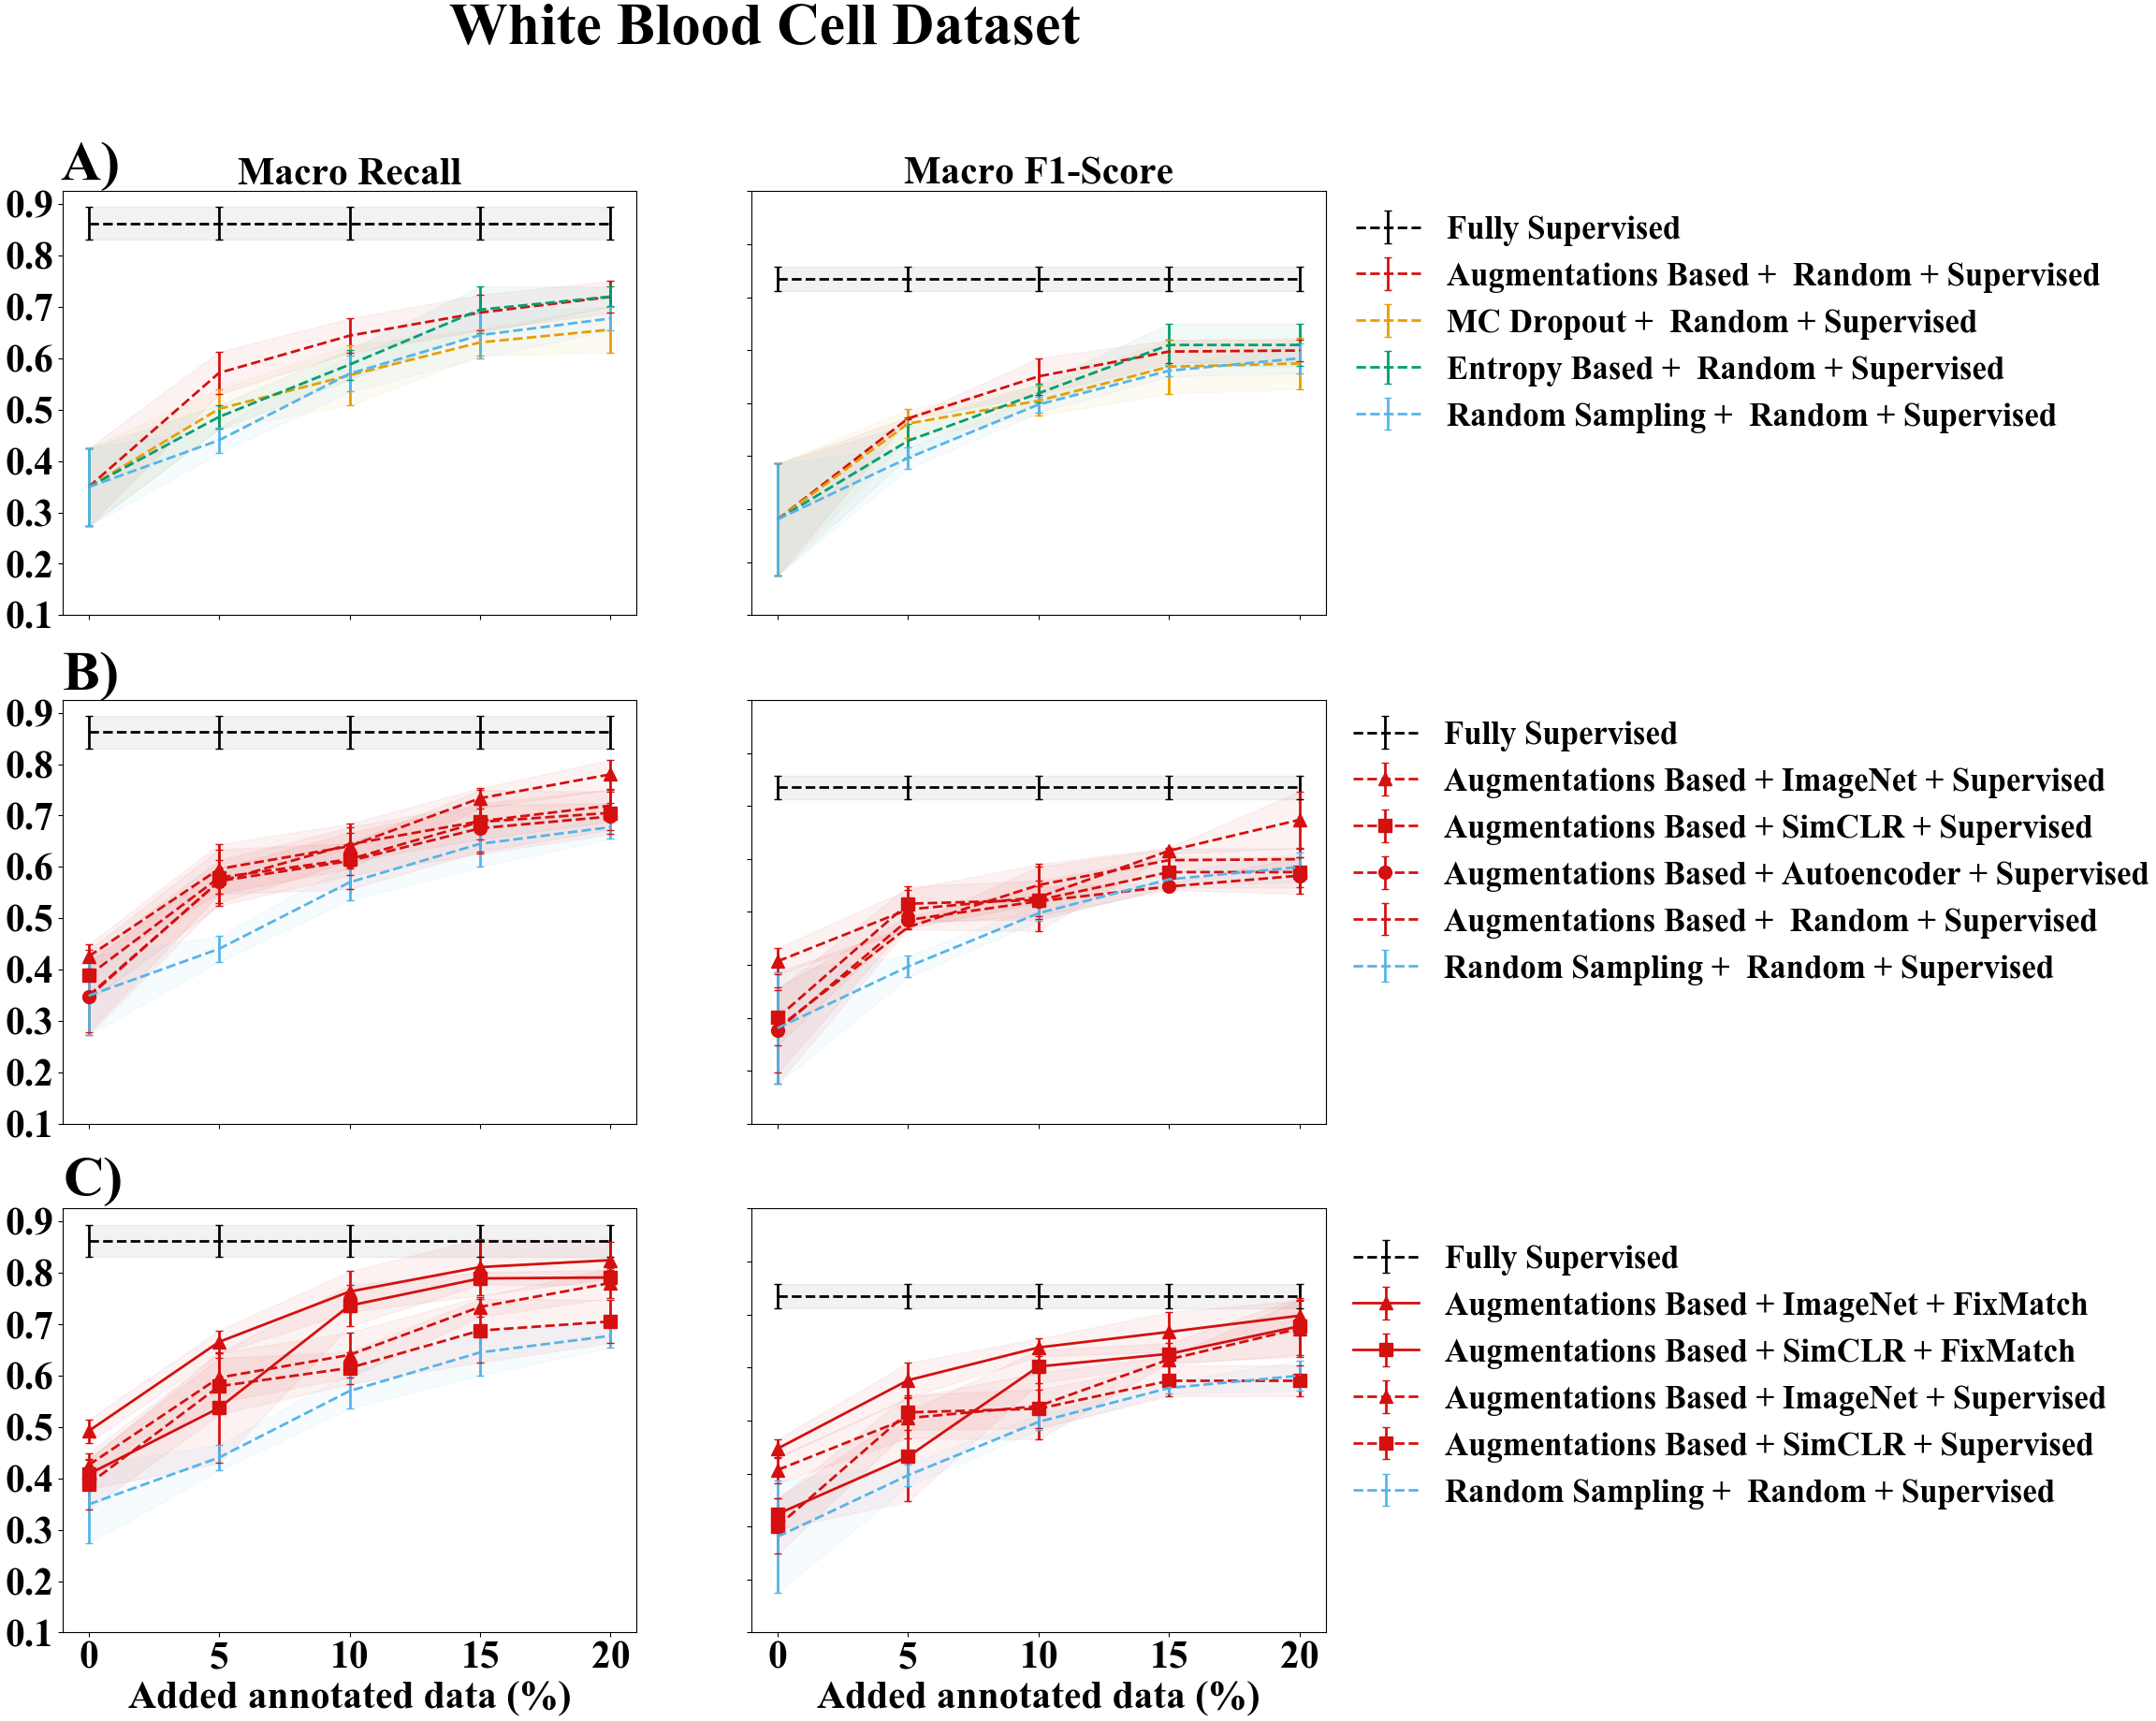
\includegraphics[width=\textwidth]{figures/fig_2_white_recall_f1.png}
\caption{In case of white blood cell dataset, the combination of augmentation-based sampling, pre-trained ImageNet weights pre-training and semi-supervised learning using FixMatch results in a performance which converges to fully-supervised learning. (A) Macro recall and macro f1-score is depicted for 3 active learning algorithms. The dashed red line represents augmentation-based sampling, dashed green line represents the entropy-based sampling, dashed yellow line shows MC-dropout and the dashed blue line show random sampling. 1\% of data is used initially and 5\% of the total data is added at every active learning iteration (B) The best performing active learning algorithm in terms of Macro Recall from A is augmentation-based sampling. It is chosen for making a comparison between different pre-training methods i.e. pre-trained ImageNet weights are shown with triangle markers, SimCLR with square markers and autoencoders are shown using circle markers. Random initialization with random sampling is shown as a dashed blue line. (C) For showing the effect of adding semi-supervised learning, FixMatch is used in conjunction with the best performing algorithms from B.}
\label{fig:fig_2_white_recall_f1}
\end{figure}

\begin{figure}[htbp]
\centering
\captionsetup{format=plain}
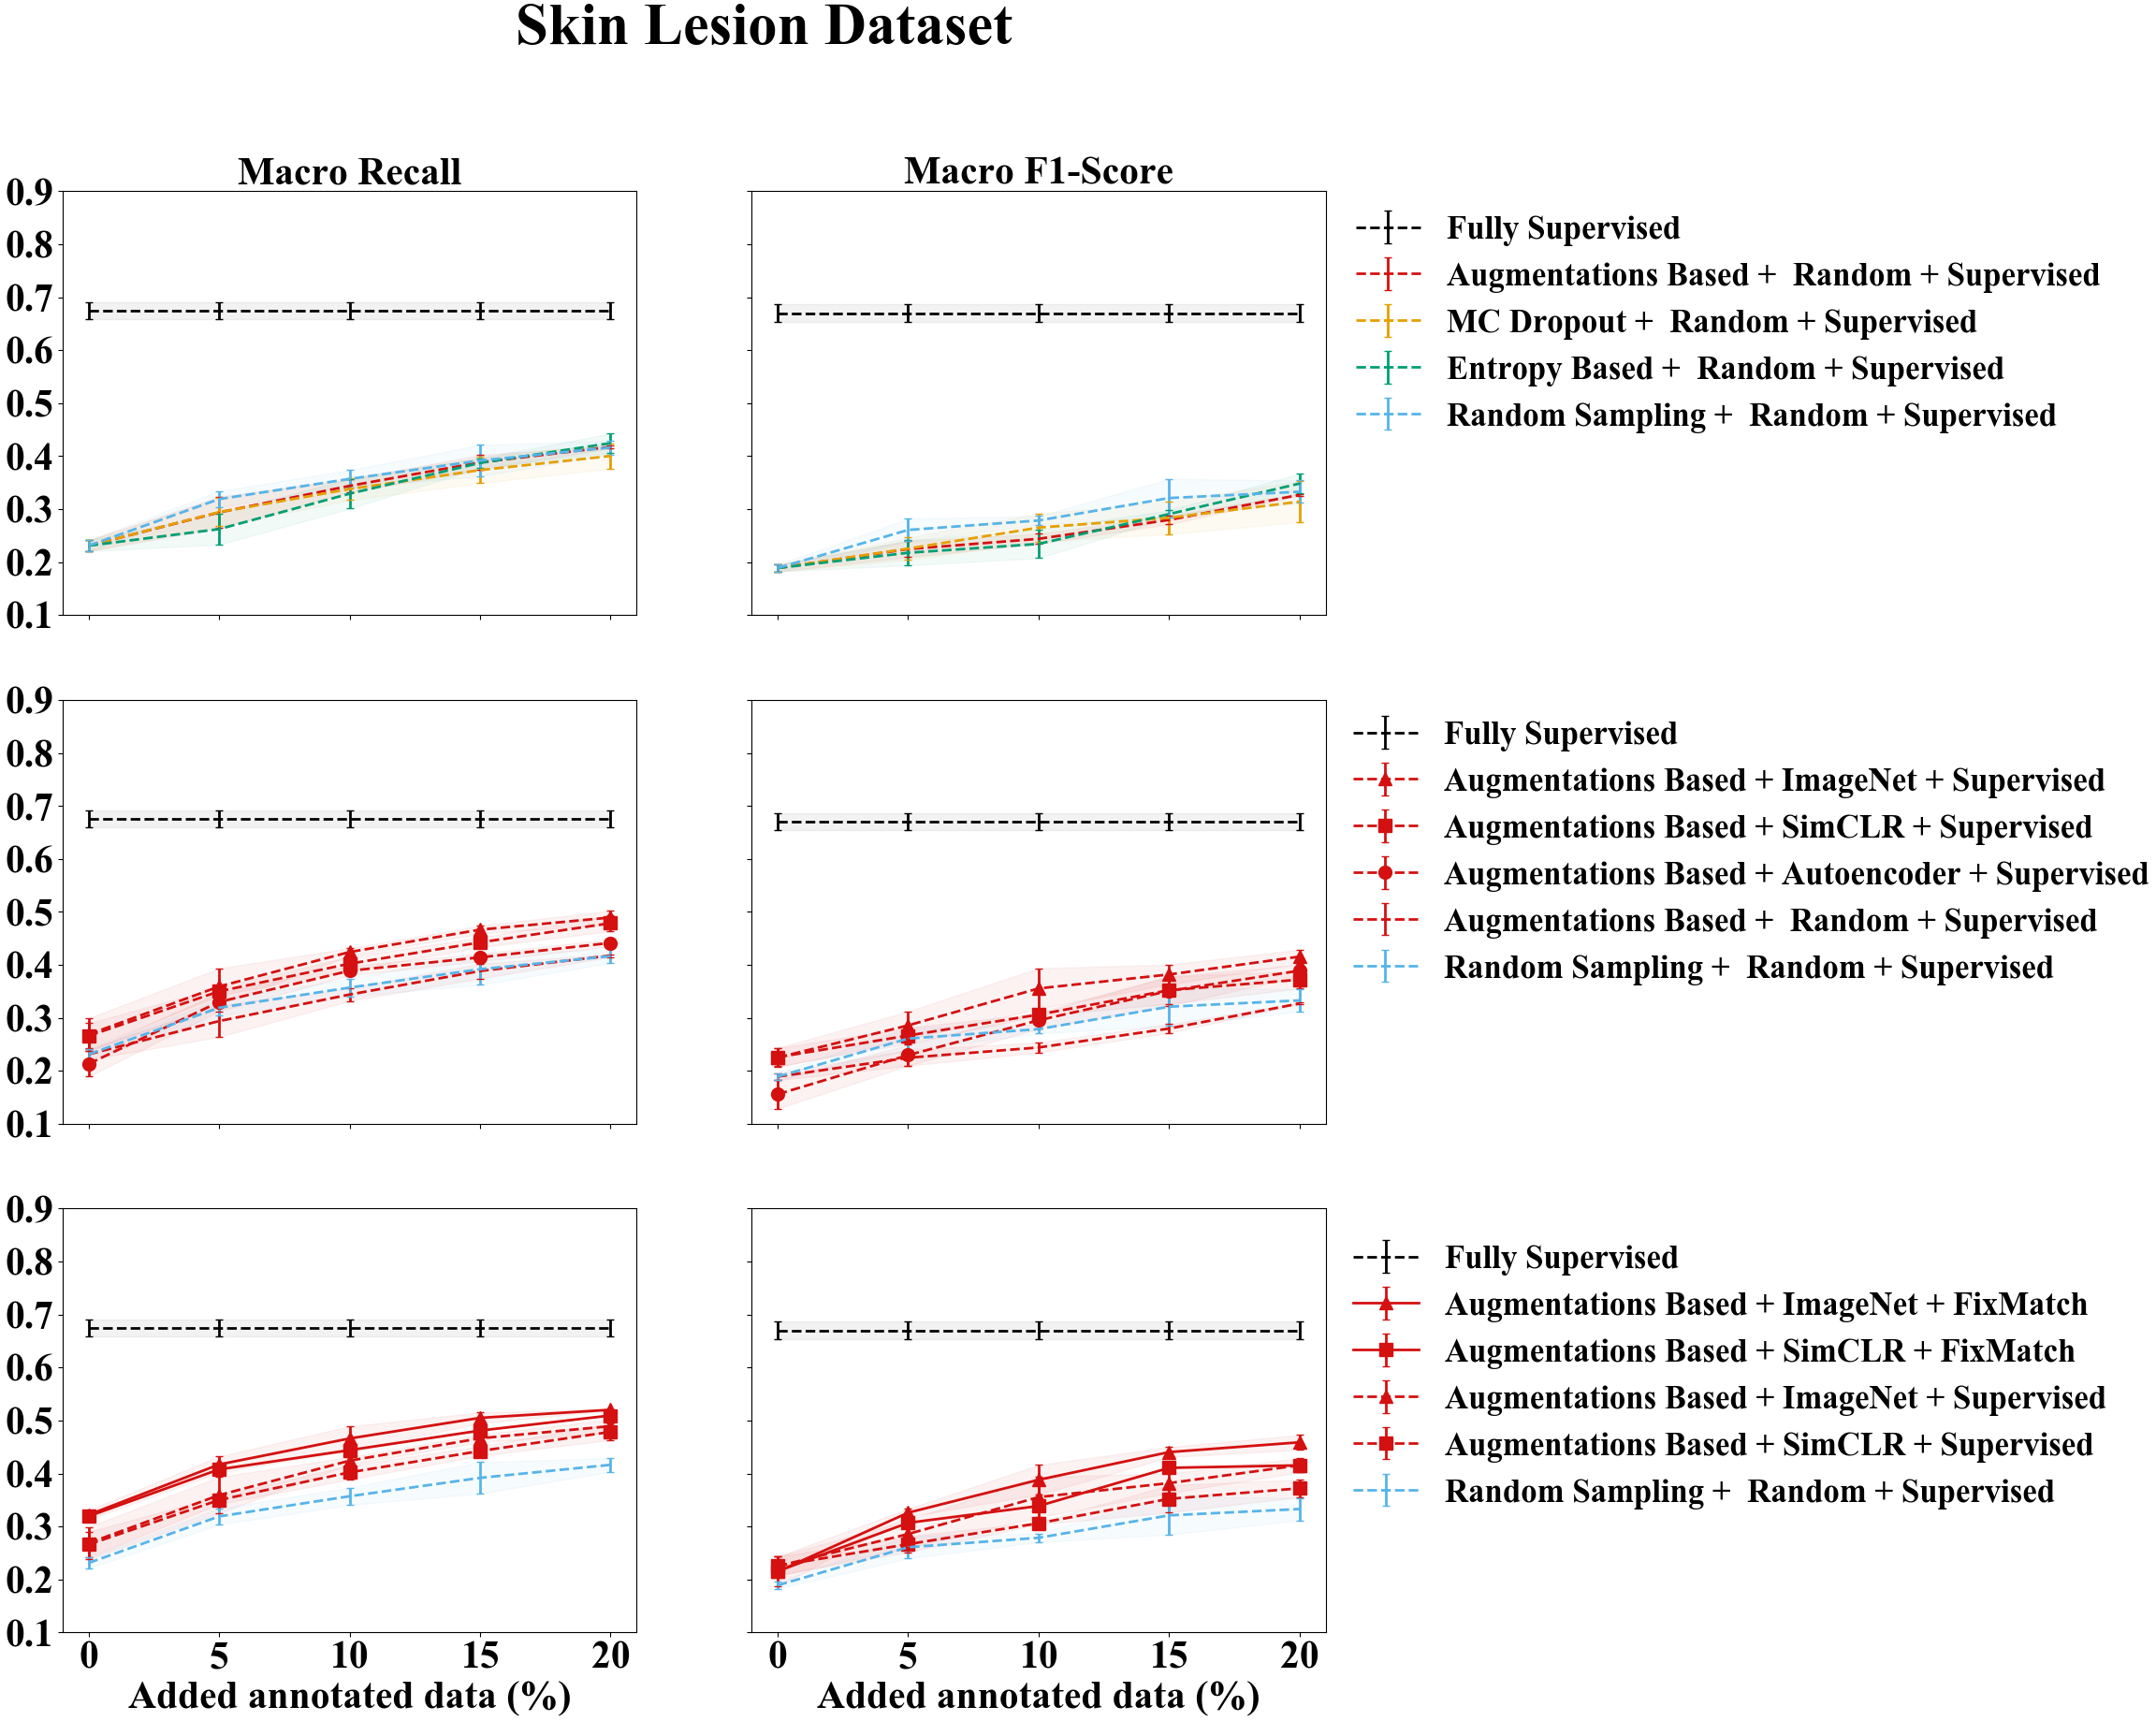
\includegraphics[width=\textwidth]{figures/fig_2_skin_recall_f1.png}
\caption{In case of the skin lesion dataset, the combination of augmentation-based sampling, pre-trained ImageNet weights pre-training and semi-supervised learning is the best performing combination but the performance does not approach fully-supervised learning performance. (A) The figure depicts the macro recall and macro f1-score for the three active learning algorithms in addition to random sampling. All of the algorithms achieve similar performance for skin lesion dataset.(B) As mentioned in A, all active learning algorithms perform similarly. However, as augmentation is shown to be the best performing active learning algorithm (Figure \ref{fig:results_3}) for skin lesion dataset during the extensive grid search, augmentation-based sampling's  performance for different pre-training methods has been shown. Pre-training using pre-trained ImageNet weights shows the best performance in terms of Macro Recall and Macro F1-score. (C) Lastly, to show the effect of semi-supervised learning, the best performing combination from B are selected and tested after the addition of FixMatch.}
\label{fig:fig_2_skin_recall_f1}
\end{figure}

\begin{figure}[htbp]
\centering
\captionsetup{format=plain}
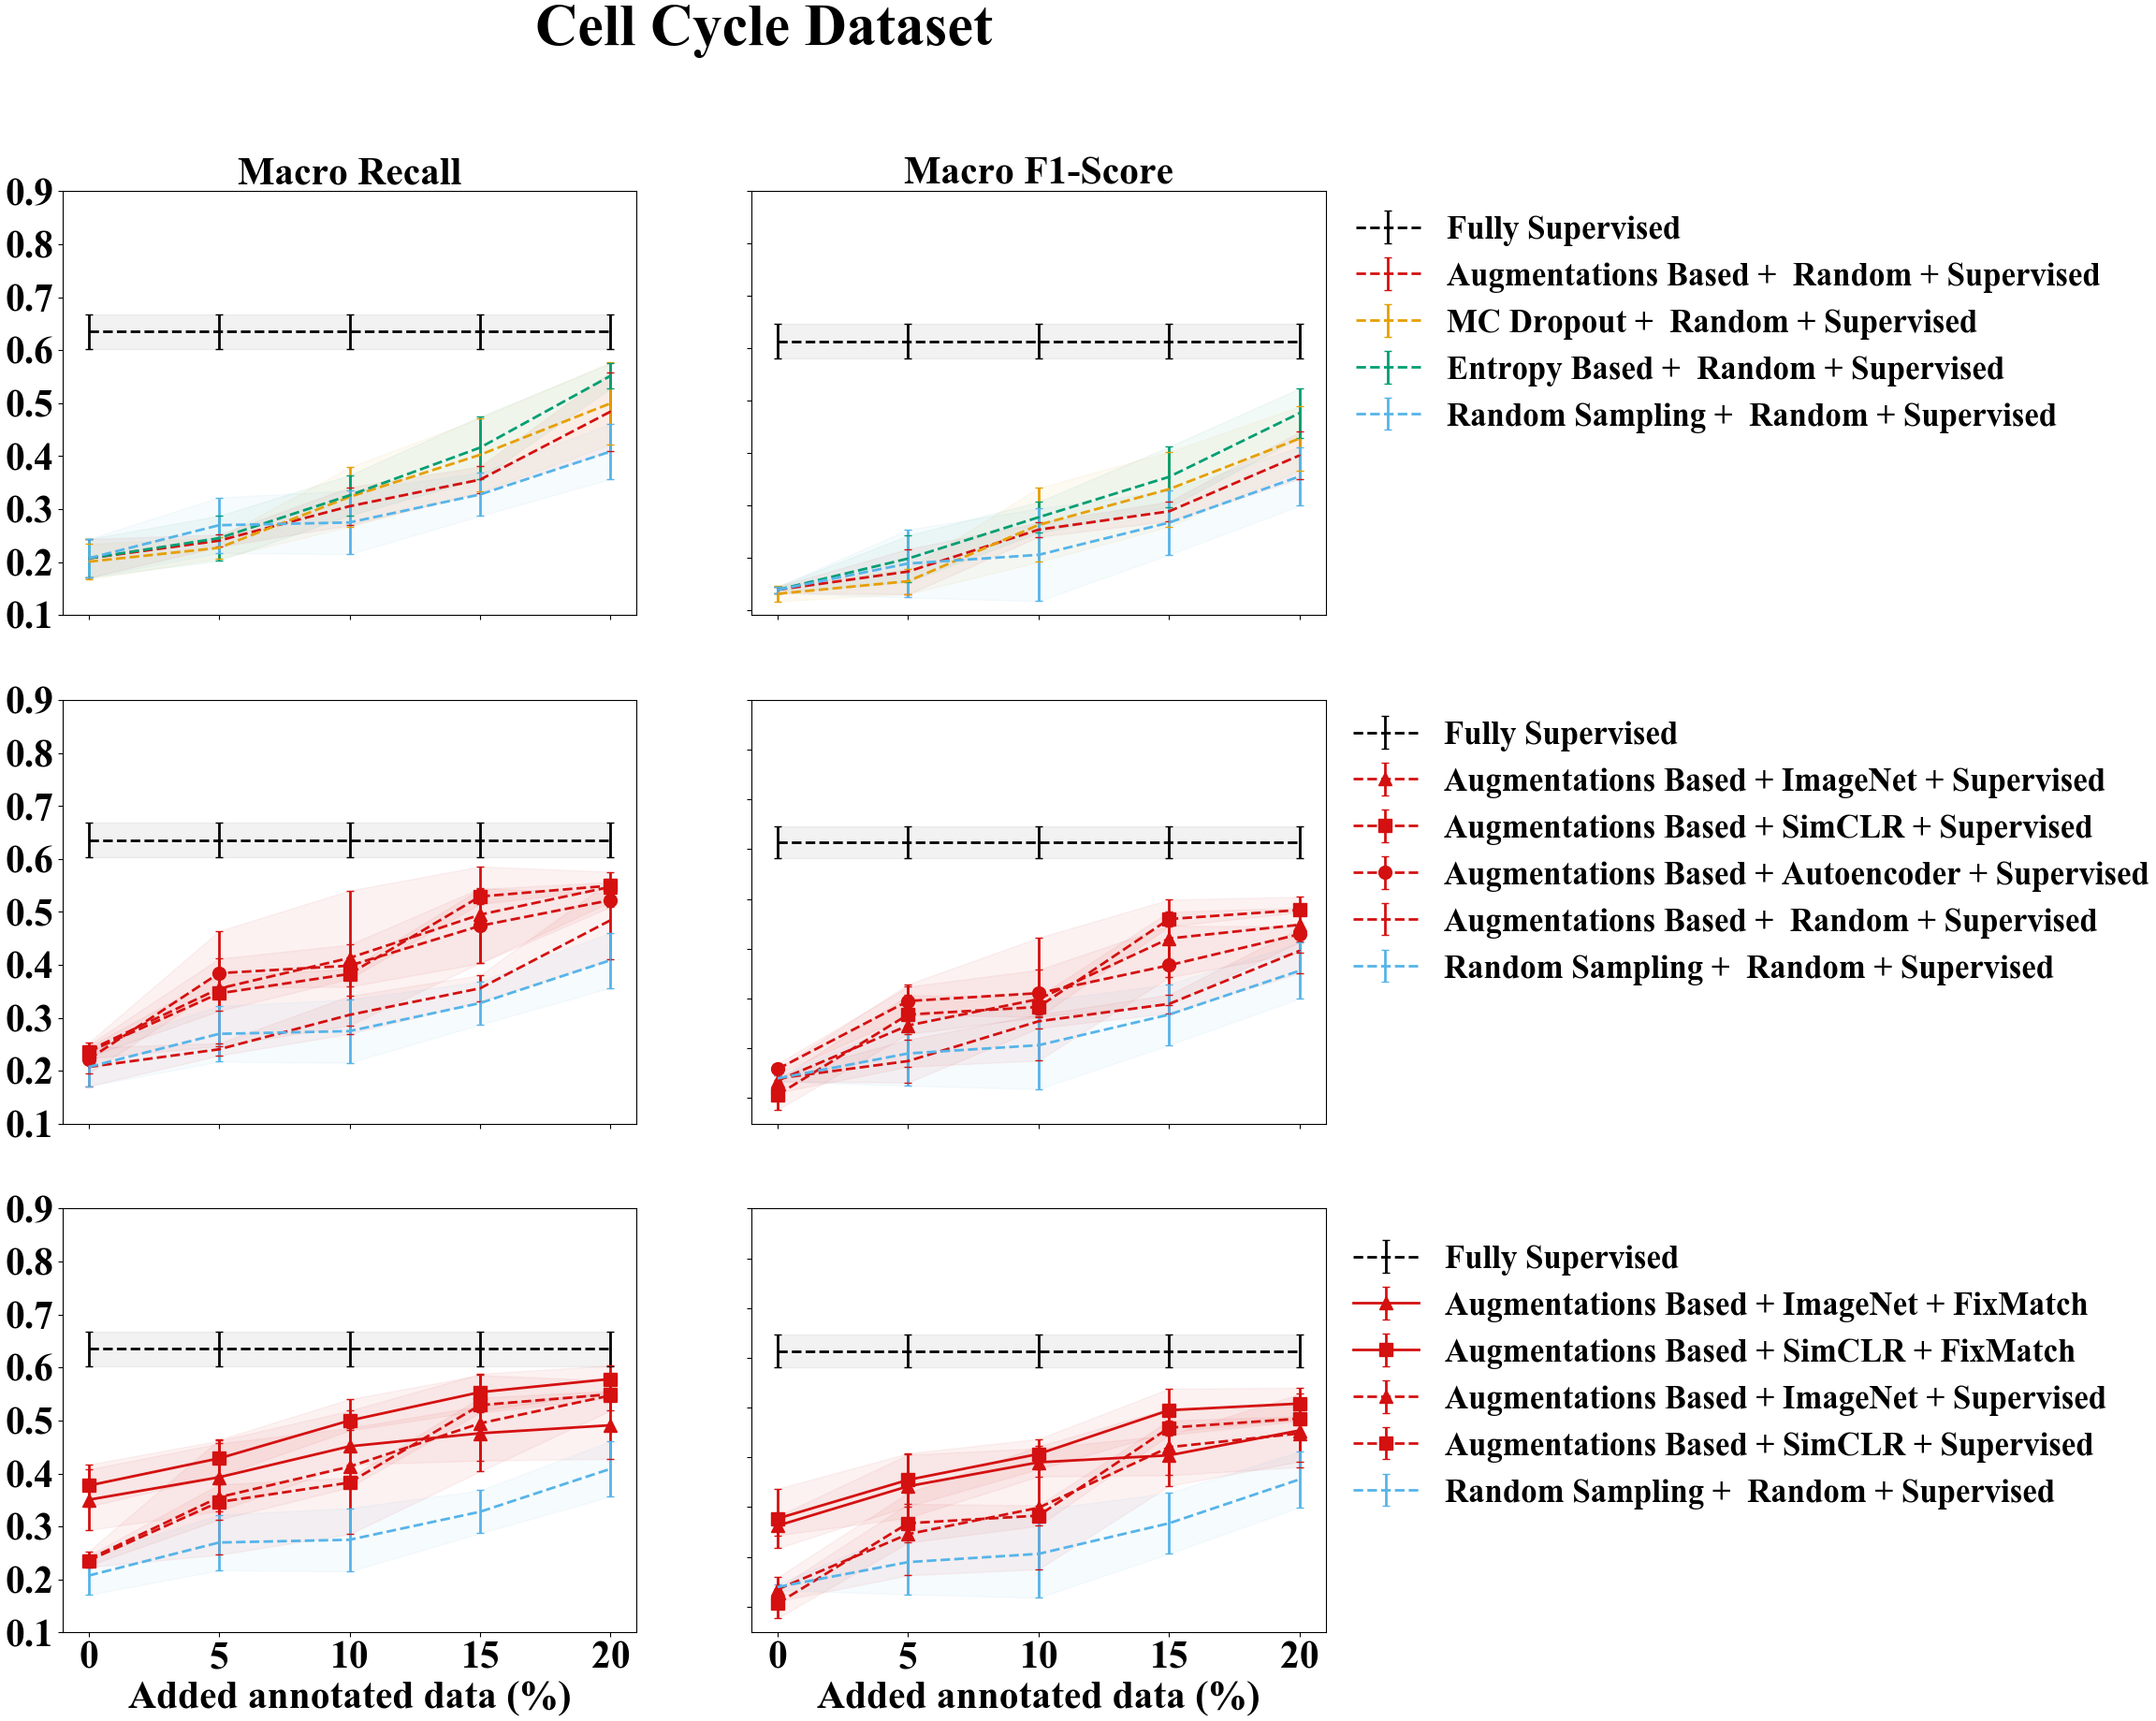
\includegraphics[width=\textwidth]{figures/fig_2_cycle_recall_f1.png}
\caption{In case of the cell cycle dataset, the combination of augmentation-based sampling, SimCLR pre-training and semi-supervised learning using FixMatch approaches the performance of fully-supervised learning on full dataset. (A) Macro recall and macro f1-score are shown for different active learning algorithms. For cell cycle dataset, entropy-based sampling is the best performing algorithm. MC-dropout and augmentation-based sampling show similar performance. All algorithms perform better than random sampling. (B) Although, entropy-based sampling is the best performing active learning algorithm. It is shown (Figure \ref{fig:results_3}), that augmentation-based sampling performs the best when pre-training and semi-supervised learning is added. Hence, augmentation-based sampling is chosen for showing the effect on performance of using different pre-training methods. (C) FixMatch is added, to test the results after adding semi-supervised learning.}
\label{fig:fig_2_cycle_recall_f1}
\end{figure}

\begin{figure}[htbp]
\centering
\captionsetup{format=plain}
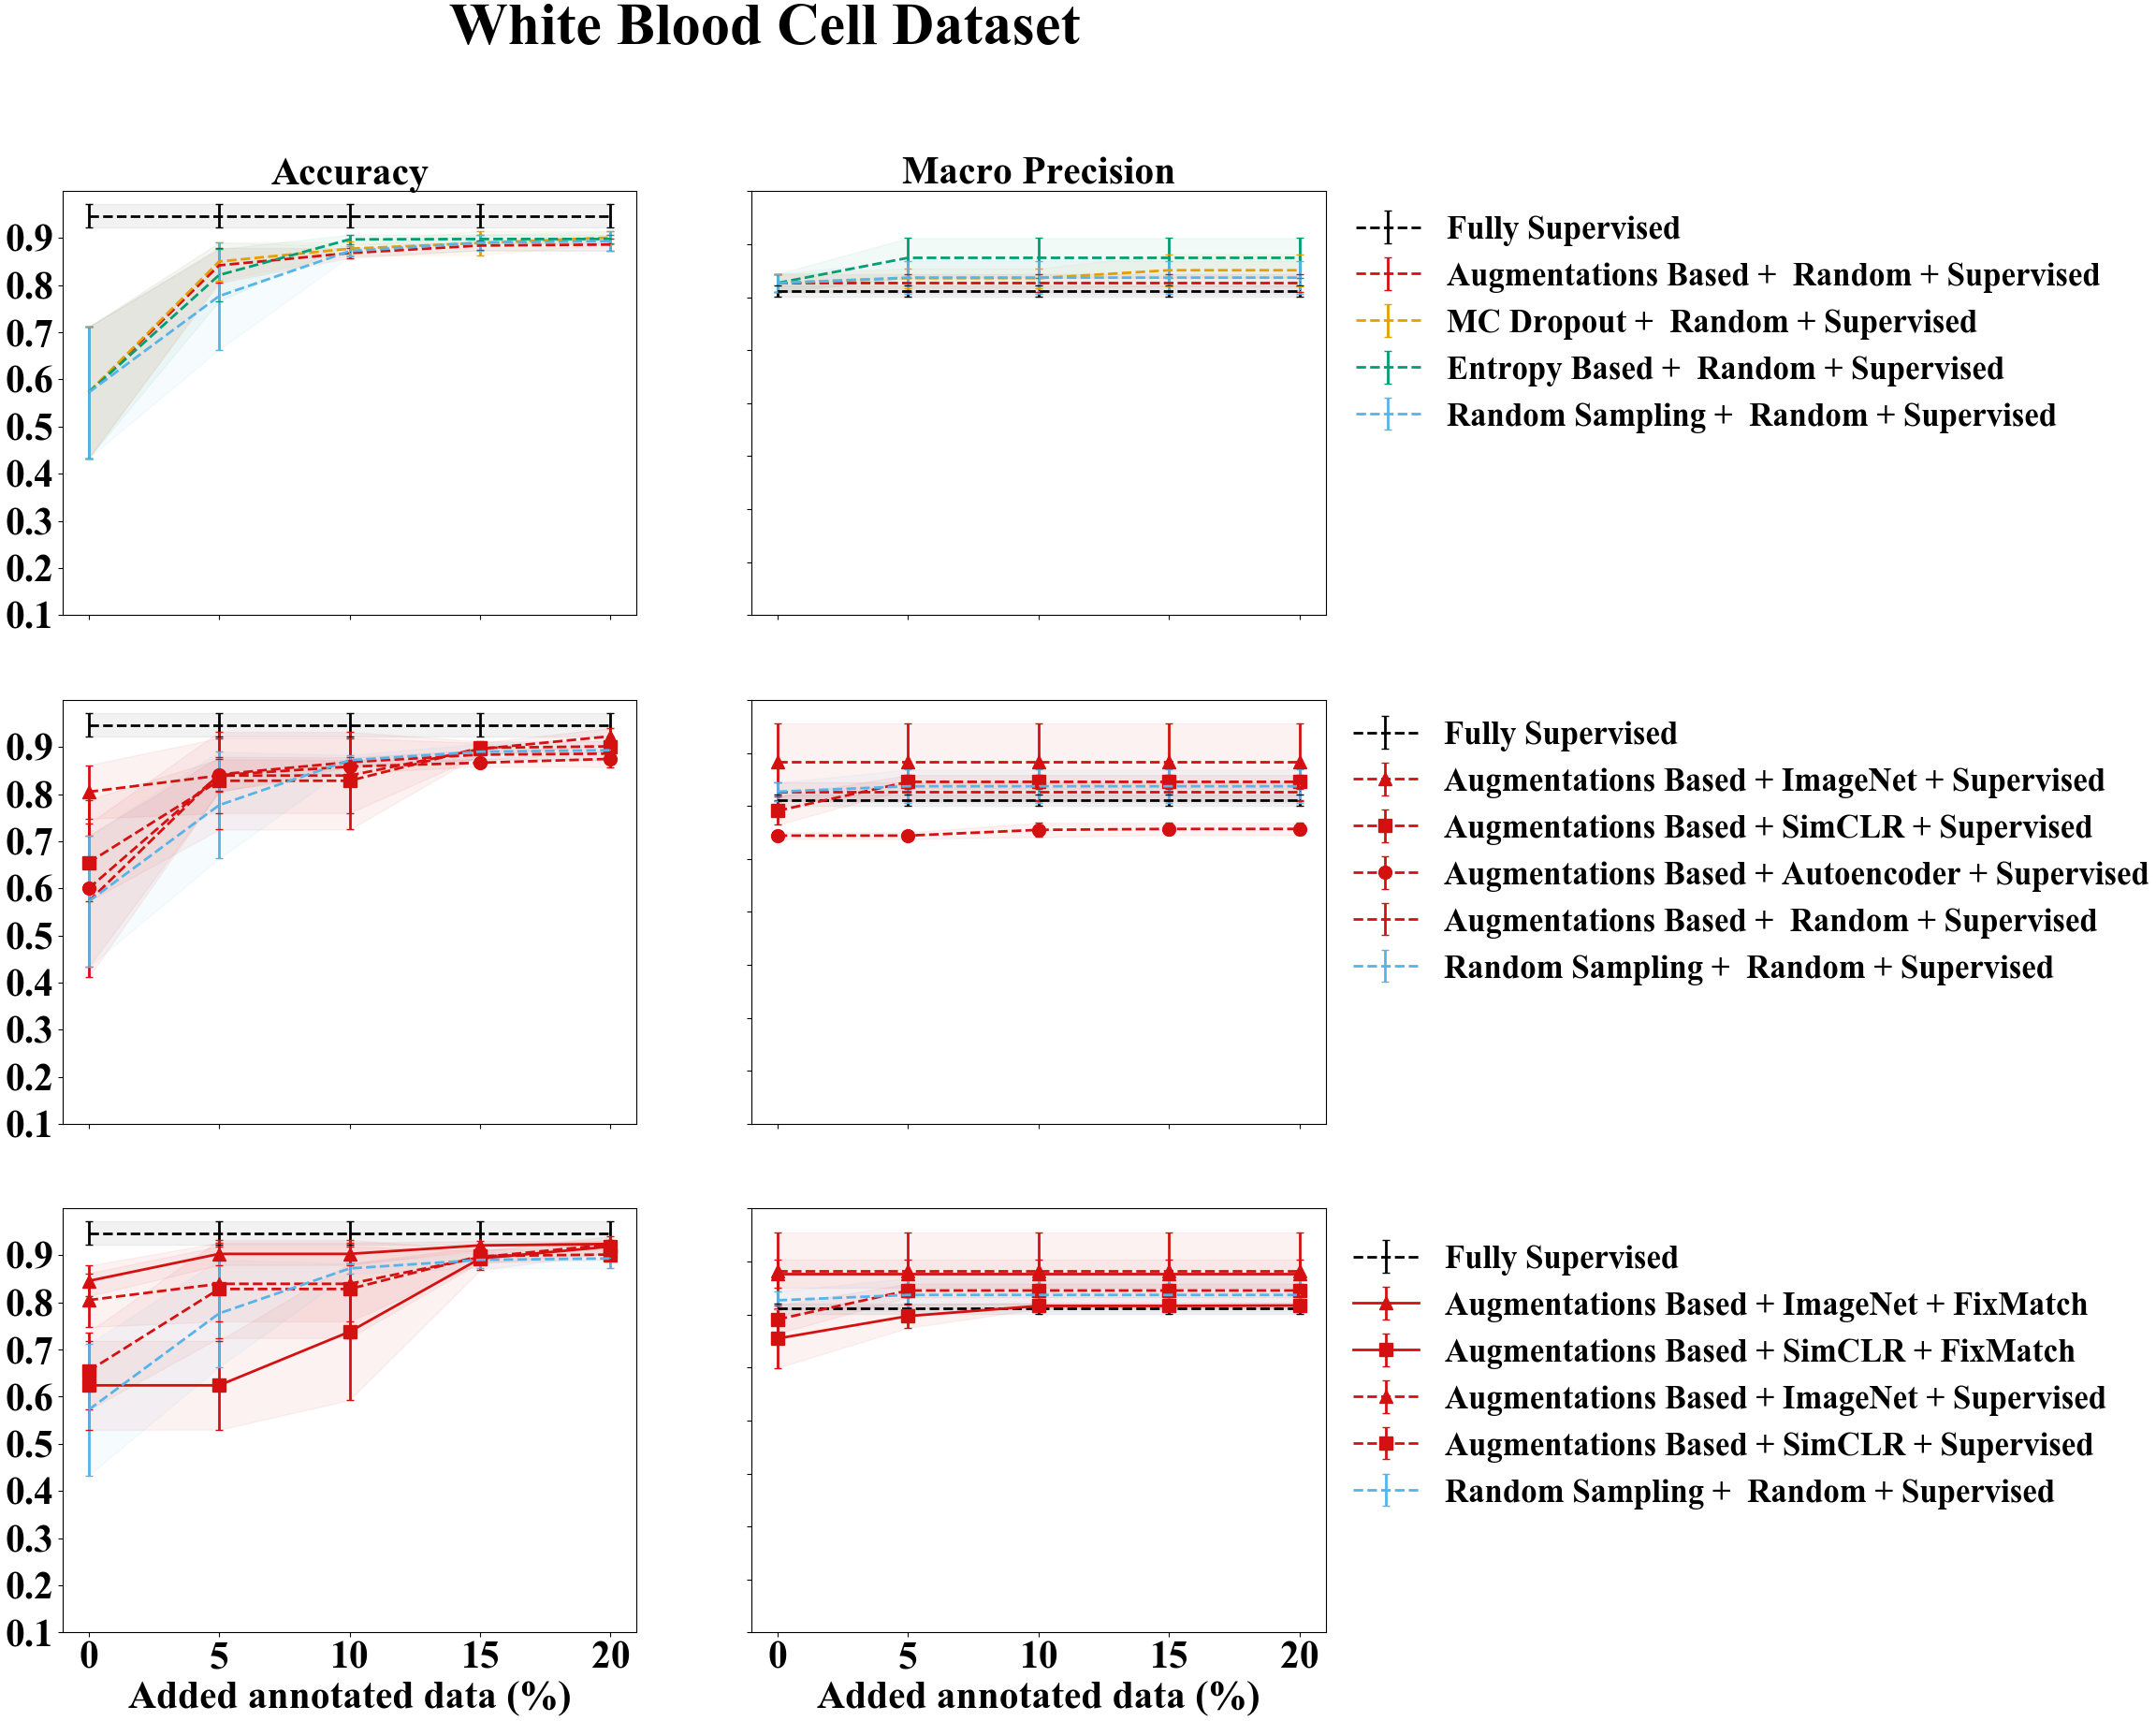
\includegraphics[width=\textwidth]{figures/fig_2_white_acc_precision.png}
\caption{On the white blood cell dataset, combining augmentation-based sampling, ImageNet pre-training and semi-supervised learning via FixMatch converges to the performance of fully-supervised learning. (A) Macro recall for 3 different active learning algorithms is computed, including augmentation-based sampling (dashed red line) entropy-based sampling (dashed green line), and MC-dropout (dashed yellow line) and a comparison is made to random sampling (dashed blue line). 1\% of the data is used as the initial labeled set. In each iteration, 5\% of data is added to the labeled set. Mean $\pm$ standard deviation of the macro recall is shown after 4-fold cross-validation. (B) Augmentation-based sampling (dashed red line, as in A) is chosen as the best active learning algorithm and a comparison is made using different pre-training methods including ImageNet weights (triangle), SimCLR (square), and autoencoder (circle) with random initialization (dashed blue line). (C) To study the effect of semi-supervised learning, the best performing experiments from B are repeated using FixMatch.}
\label{fig:fig_2_white_acc_precision}
\end{figure}

\begin{figure}[htbp]
\centering
\captionsetup{format=plain}
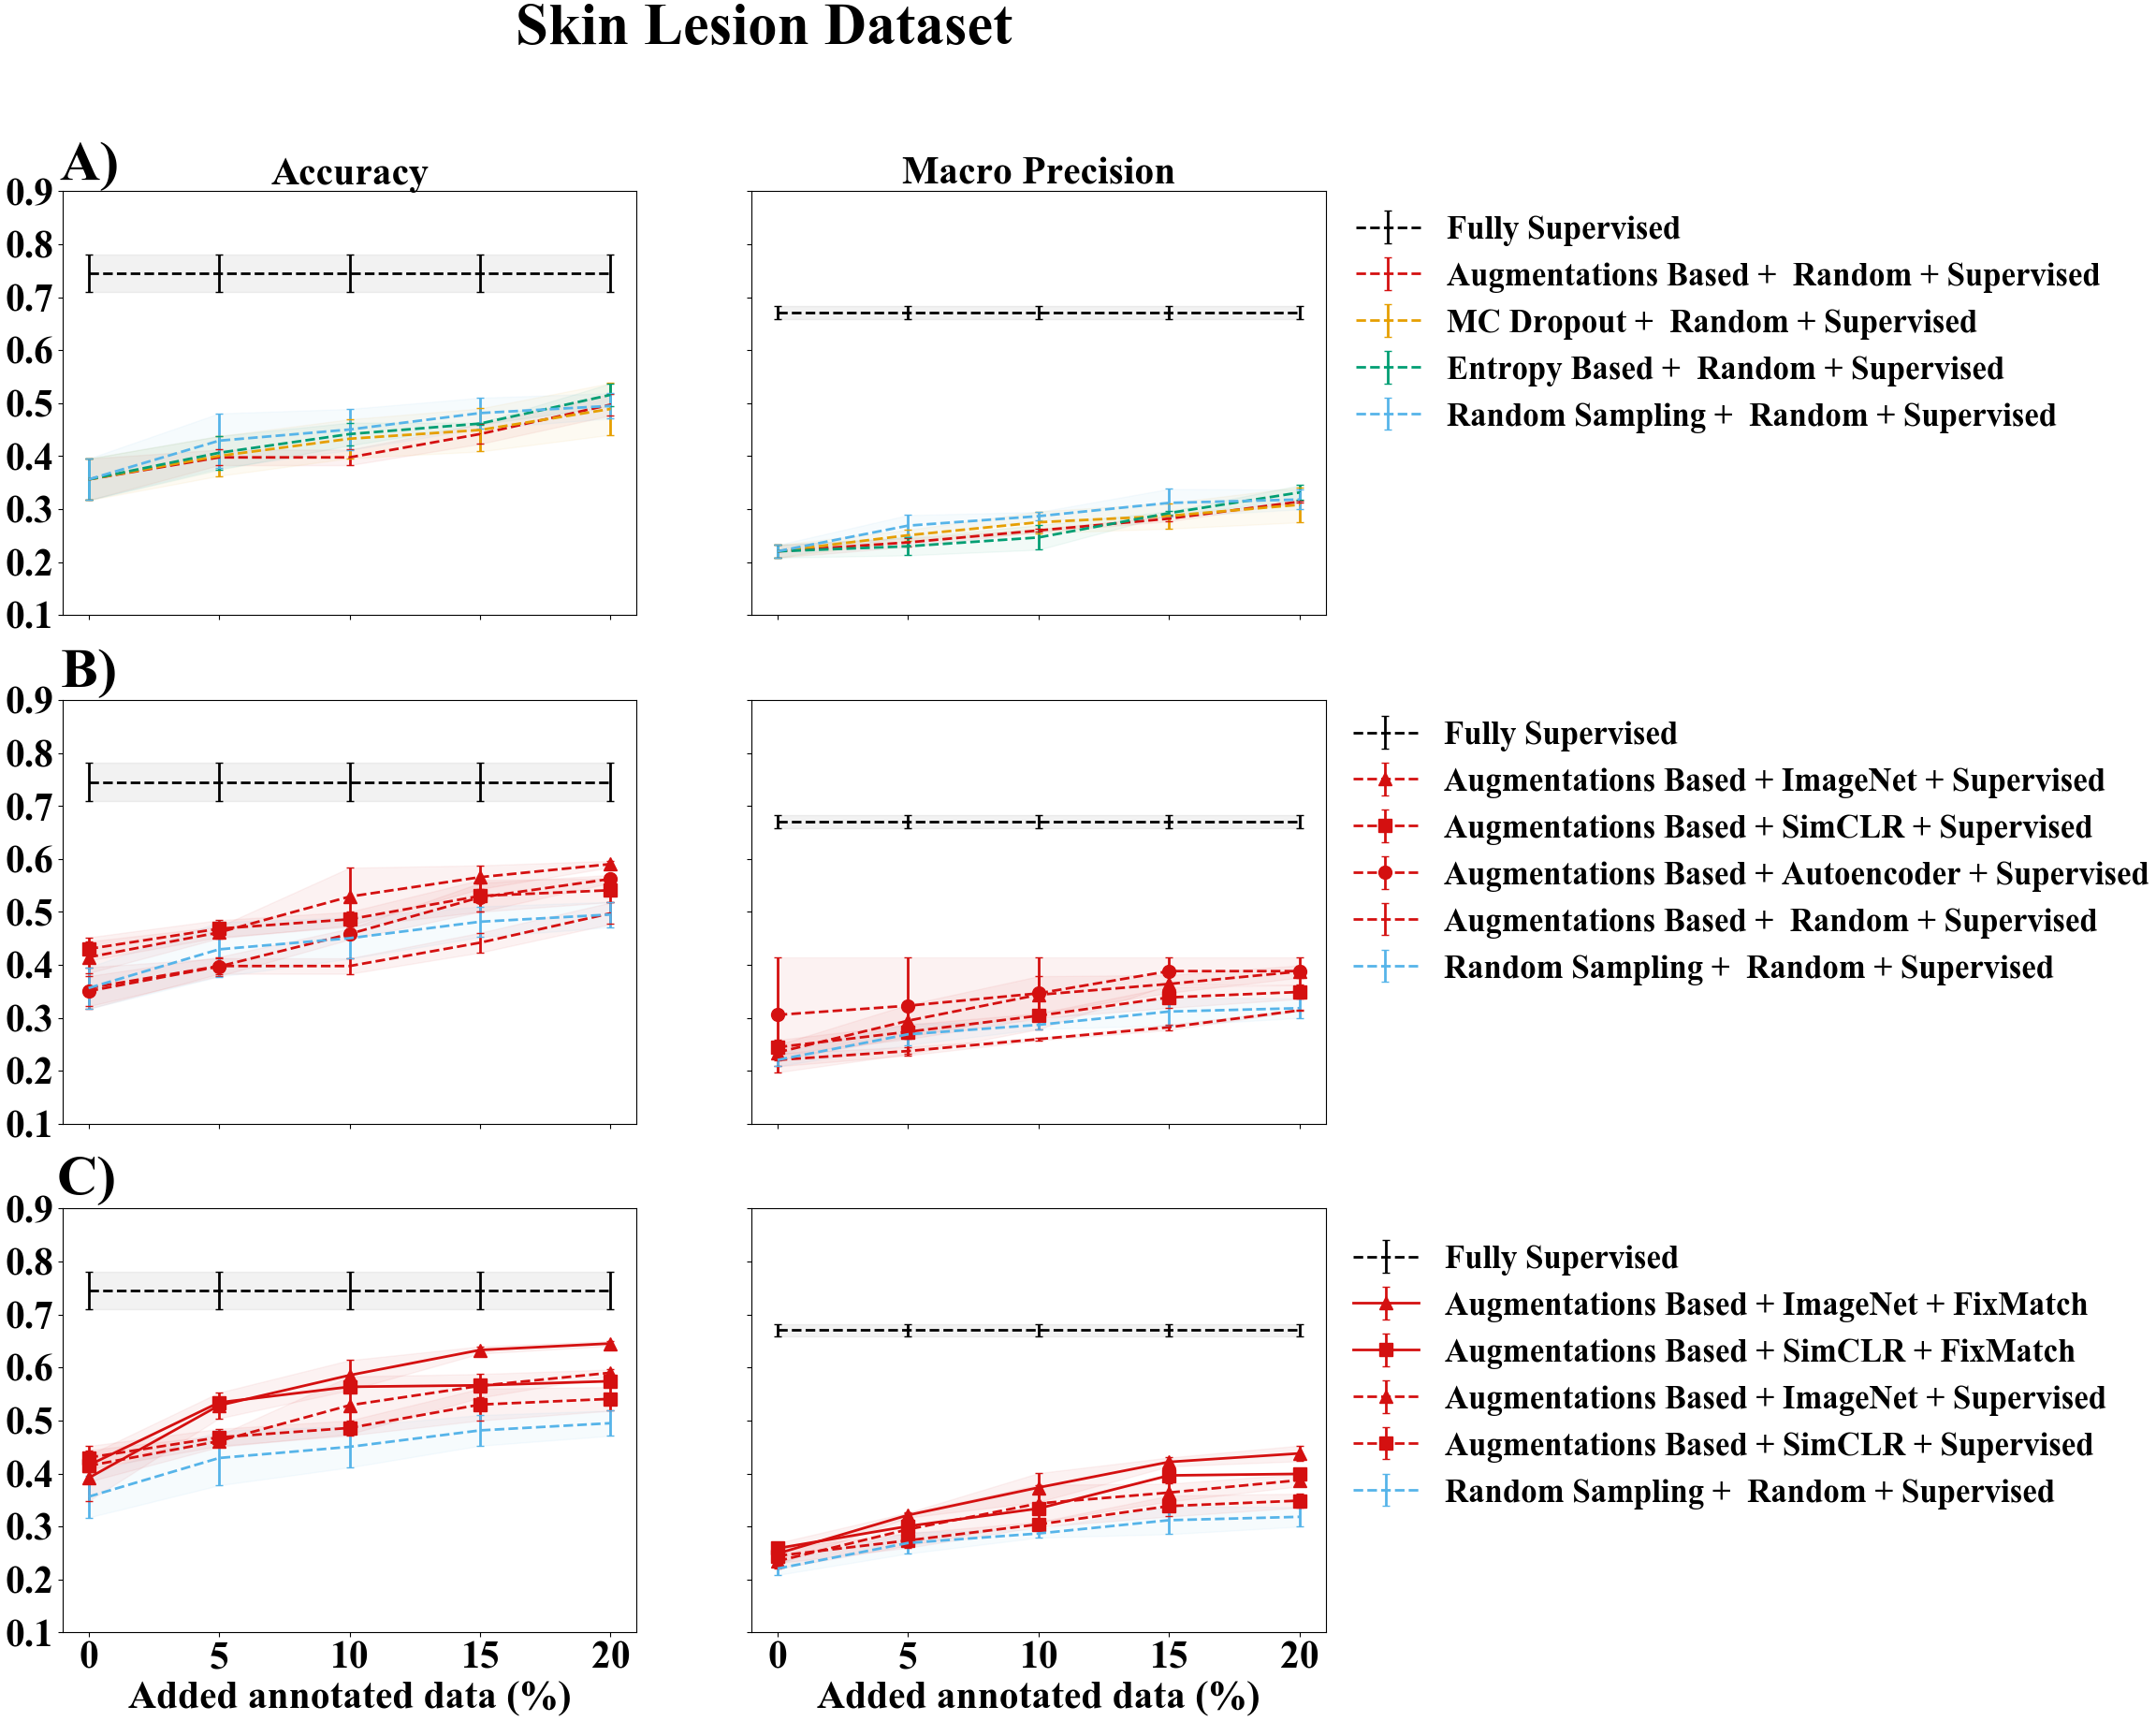
\includegraphics[width=\textwidth]{figures/fig_2_skin_acc_precision.png}
\caption{On the white blood cell dataset, combining augmentation-based sampling, ImageNet pre-training and semi-supervised learning via FixMatch converges to the performance of fully-supervised learning. (A) Macro recall for 3 different active learning algorithms is computed, including augmentation-based sampling (dashed red line) entropy-based sampling (dashed green line), and MC-dropout (dashed yellow line) and a comparison is made to random sampling (dashed blue line). 1\% of the data is used as the initial labeled set. In each iteration, 5\% of data is added to the labeled set. Mean $\pm$ standard deviation of the macro recall is shown after 4-fold cross-validation. (B) Augmentation-based sampling (dashed red line, as in A) is chosen as the best active learning algorithm and a comparison is made using different pre-training methods including ImageNet weights (triangle), SimCLR (square), and autoencoder (circle) with random initialization (dashed blue line). (C) To study the effect of semi-supervised learning, the best performing experiments from B are repeated using FixMatch.}
\label{fig:fig_2_skin_acc_precision}
\end{figure}

\begin{figure}[htbp]
\centering
\captionsetup{format=plain}
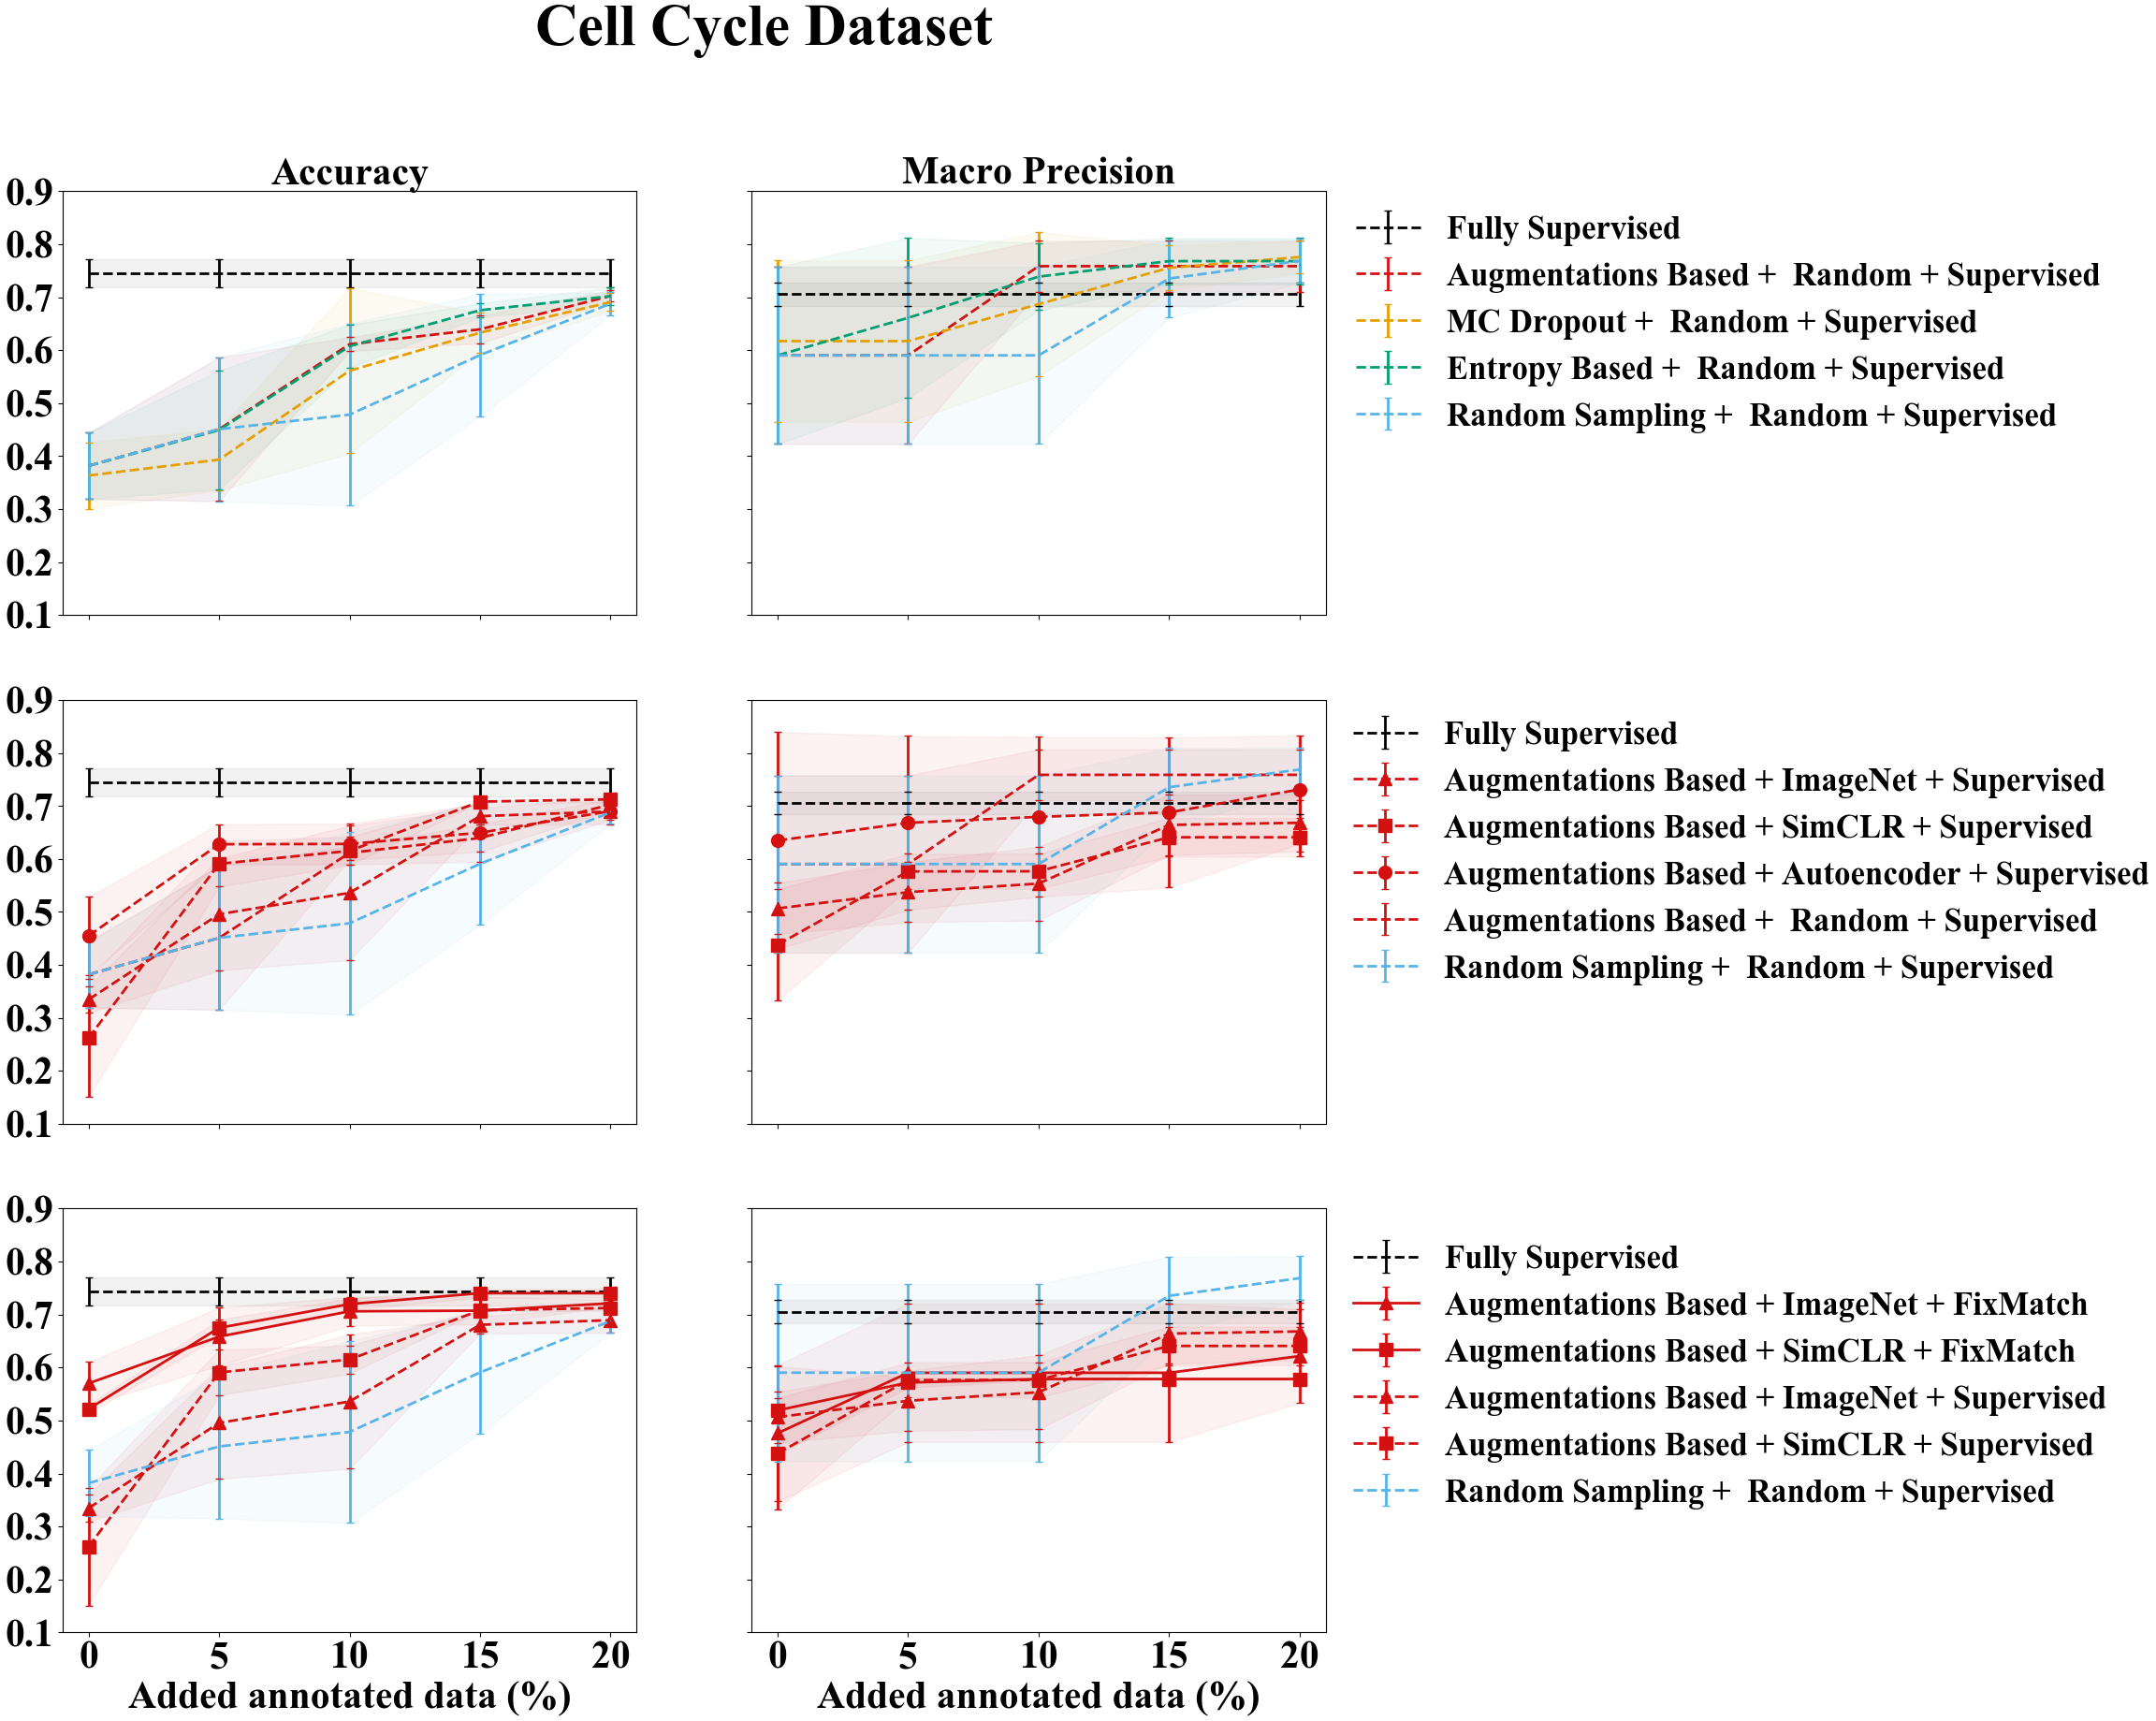
\includegraphics[width=\textwidth]{figures/fig_2_cycle_acc_precision.png}
\caption{On the white blood cell dataset, combining augmentation-based sampling, ImageNet pre-training and semi-supervised learning via FixMatch converges to the performance of fully-supervised learning. (A) Macro recall for 3 different active learning algorithms is computed, including augmentation-based sampling (dashed red line) entropy-based sampling (dashed green line), and MC-dropout (dashed yellow line) and a comparison is made to random sampling (dashed blue line). 1\% of the data is used as the initial labeled set. In each iteration, 5\% of data is added to the labeled set. Mean $\pm$ standard deviation of the macro recall is shown after 4-fold cross-validation. (B) Augmentation-based sampling (dashed red line, as in A) is chosen as the best active learning algorithm and a comparison is made using different pre-training methods including ImageNet weights (triangle), SimCLR (square), and autoencoder (circle) with random initialization (dashed blue line). (C) To study the effect of semi-supervised learning, the best performing experiments from B are repeated using FixMatch.}
\label{fig:fig_2_cycle_acc_precision}
\end{figure}

\section{Comparison of active learning algorithms on white blood cell data}
First, the performance of different annotation-efficient approaches is compared on the white blood cell dataset (Figure \ref{fig:fig_2_white_recall_f1}). Random Initialization is used for model weights initialization and the model is trained under the supervised learning paradigm i.e. using labeled data only. The augmentation-based sampling achieves better performance compared to all other active learning algorithms (see Figure \ref{fig:results_3}) in almost all active learning iterations (see Figure \ref{fig:fig_2_white_recall_f1}). At the last active learning iteration, after 20\% of data has already been added to the labeled set $\mathcal{L}$ as annotated images, the augmentation-based sampling has a macro recall of 0.72$\pm$0.03, entropy-based sampling a macro recall of 0.72$\pm$0.02, MC-dropout a recall of 0.66$\pm$0.04 and random sampling a recall of 0.68$\pm$0.02.

\section{Pre-training on white blood cell images further improves performance}
Augmentation-based sampling is the best performing active learning algorithm. The performance obtained through augmentation sampling is further improved by adding pre-training (Figure \ref{fig:fig_2_white_recall_f1}). Using augmentation-based sampling as the active learning algorithm, the experiment is repeated with three pre-training methods: using pre-trained ImageNet weights, using Autoencoder and using SimCLR (see chapter \ref{chapter:methods} and Table \ref{table:experimental_grid}). It is found that using pre-trained ImageNet  weights and SimCLR for pre-training results in a boost in performance in the first two active learning iterations with a increase of 12\% of macro recall. However, as more annotated data is added, the random initialization catches up with SimCLR and autoencoder pre-training but ImageNet pre-training still performs better than random initialization even after the addition of 20\% of the data. After the last active learning iteration, the  augmentation-based sampling with ImageNet weights reaches a macro recall of 0.78$\pm$0.03, random initialization reaches a macro recall of 0.72$\pm$0.03 and initialization with SimCLR pre-training reaches a recall of 0.71$\pm$0.04.

\section{Semi-supervised learning further improves recall for white blood cells data}
As augmentation-based sampling performed better than other active learning algorithms, it is chosen for further investigation to find out the performance improvement gained by using semi-supervised learning training strategy (Figure \ref{fig:fig_2_white_recall_f1}). The pre-training methods of using pre-trained ImageNet weights and SimCLR are used, as both of the methods performed well during the previous experiments (Figure \ref{fig:fig_2_white_recall_f1}B). For semi-supervised learning, FixMatch is used (Figure \ref{fig:fig_2_white_recall_f1}C). After adding semi-supervised learning with augmentations, a macro recall improvement of at least 6\% is observed for all iterations. This combination performs better than supervised training in each iteration and achieves a macro recall of 0.82$\pm$0.04 at the last iteration, when 20\% of annotated data has been added to the labeled set $\mathcal{L}$. FixMatch also improves augmentation-based sampling with SimCLR pre-training, reaching 0.79$\pm$0.01 macro recall. It is to be noted that when using augmentation-based active learning algorithm with ImageNet pre-training and semi-supervised learning, the macro recall is only 4\% less than using fully-supervised learning on 100\% of the data.

\section{Grid-search identifies the best performing combinations for three biomedical datasets}
To investigation if the proposed combination of augmentation-based sampling, ImageNet pre-training and semi-supervised learning performs better than other combinations in table \ref{table:experimental_grid} for biomedical datasets which involve images containing different textures, colors and structures. The proposed combination is tested on three different biomedical datasets (Figure \ref{fig:datasets_composition}). For this purpose an extensive grid search is carried out which specifically involves, 3x4x4x2x4x5 = 1920 independent runs (3 datasets, 3 active learning algorithms plus random sampling, 3 pre-training methods plus random initialization, 2 training strategies, 4-fold cross-validation and 1 initial step plus 4 active learning iterations). The criteria for measuring the performance of different combinations is the macro recall value at the last iteration when 20\% of data has been added as annotated data.

It is found that the proposed combinations of augmentation-based sampling with ImageNet or SimCLR pre-training and FixMatch consistently outperform the rest (for comparing all the combinations, please refer to the appendix).
In case of white blood cell dataset, at the first step with 1\% of labeled data a 6\% improvement in macro recall at least is observed using FixMatch with ImageNet initialization over conventional training method with only labeled data (Figure \ref{fig:all_recall_f1}A). This improvement in performance is stable, resulting in at least 4\% increase in macro recall compared to the best result obtained through supervised learning training strategy. The same trend is observed in case of the skin lesion dataset (Figure \ref{fig:all_recall_f1}B). During the first iteration, an improvement of at least 5\% is observed compared to other supervised learning conventional methods. Although the conventional supervised learning methods approach the performance of proposed combinations as more data is added, there is still a performance gap at all iterations. Lastly, for the cell cycle dataset (Figure \ref{fig:all_recall_f1}C), the combination of SimCLR with augmentation-based sampling provides a boost of at least 16\% in the macro recall in the start over other conventional methods. The performance boost gets less as more data is added but till the last iteration when 20\% of data has been added as annotated data, the performance improvement is still at least 3\% of macro recall. 
It is to be noted that, at the last iteration, for white blood cell dataset and the cell cycle dataset, the performance of the propose combinations approach the performance of fully-supervised learning on the whole dataset. However, in case of skin lesion dataset, more labeled data has to be added to approach the performance of fully supervised learning. 

\begin{figure}[htbp]
\centering
\captionsetup{format=plain}
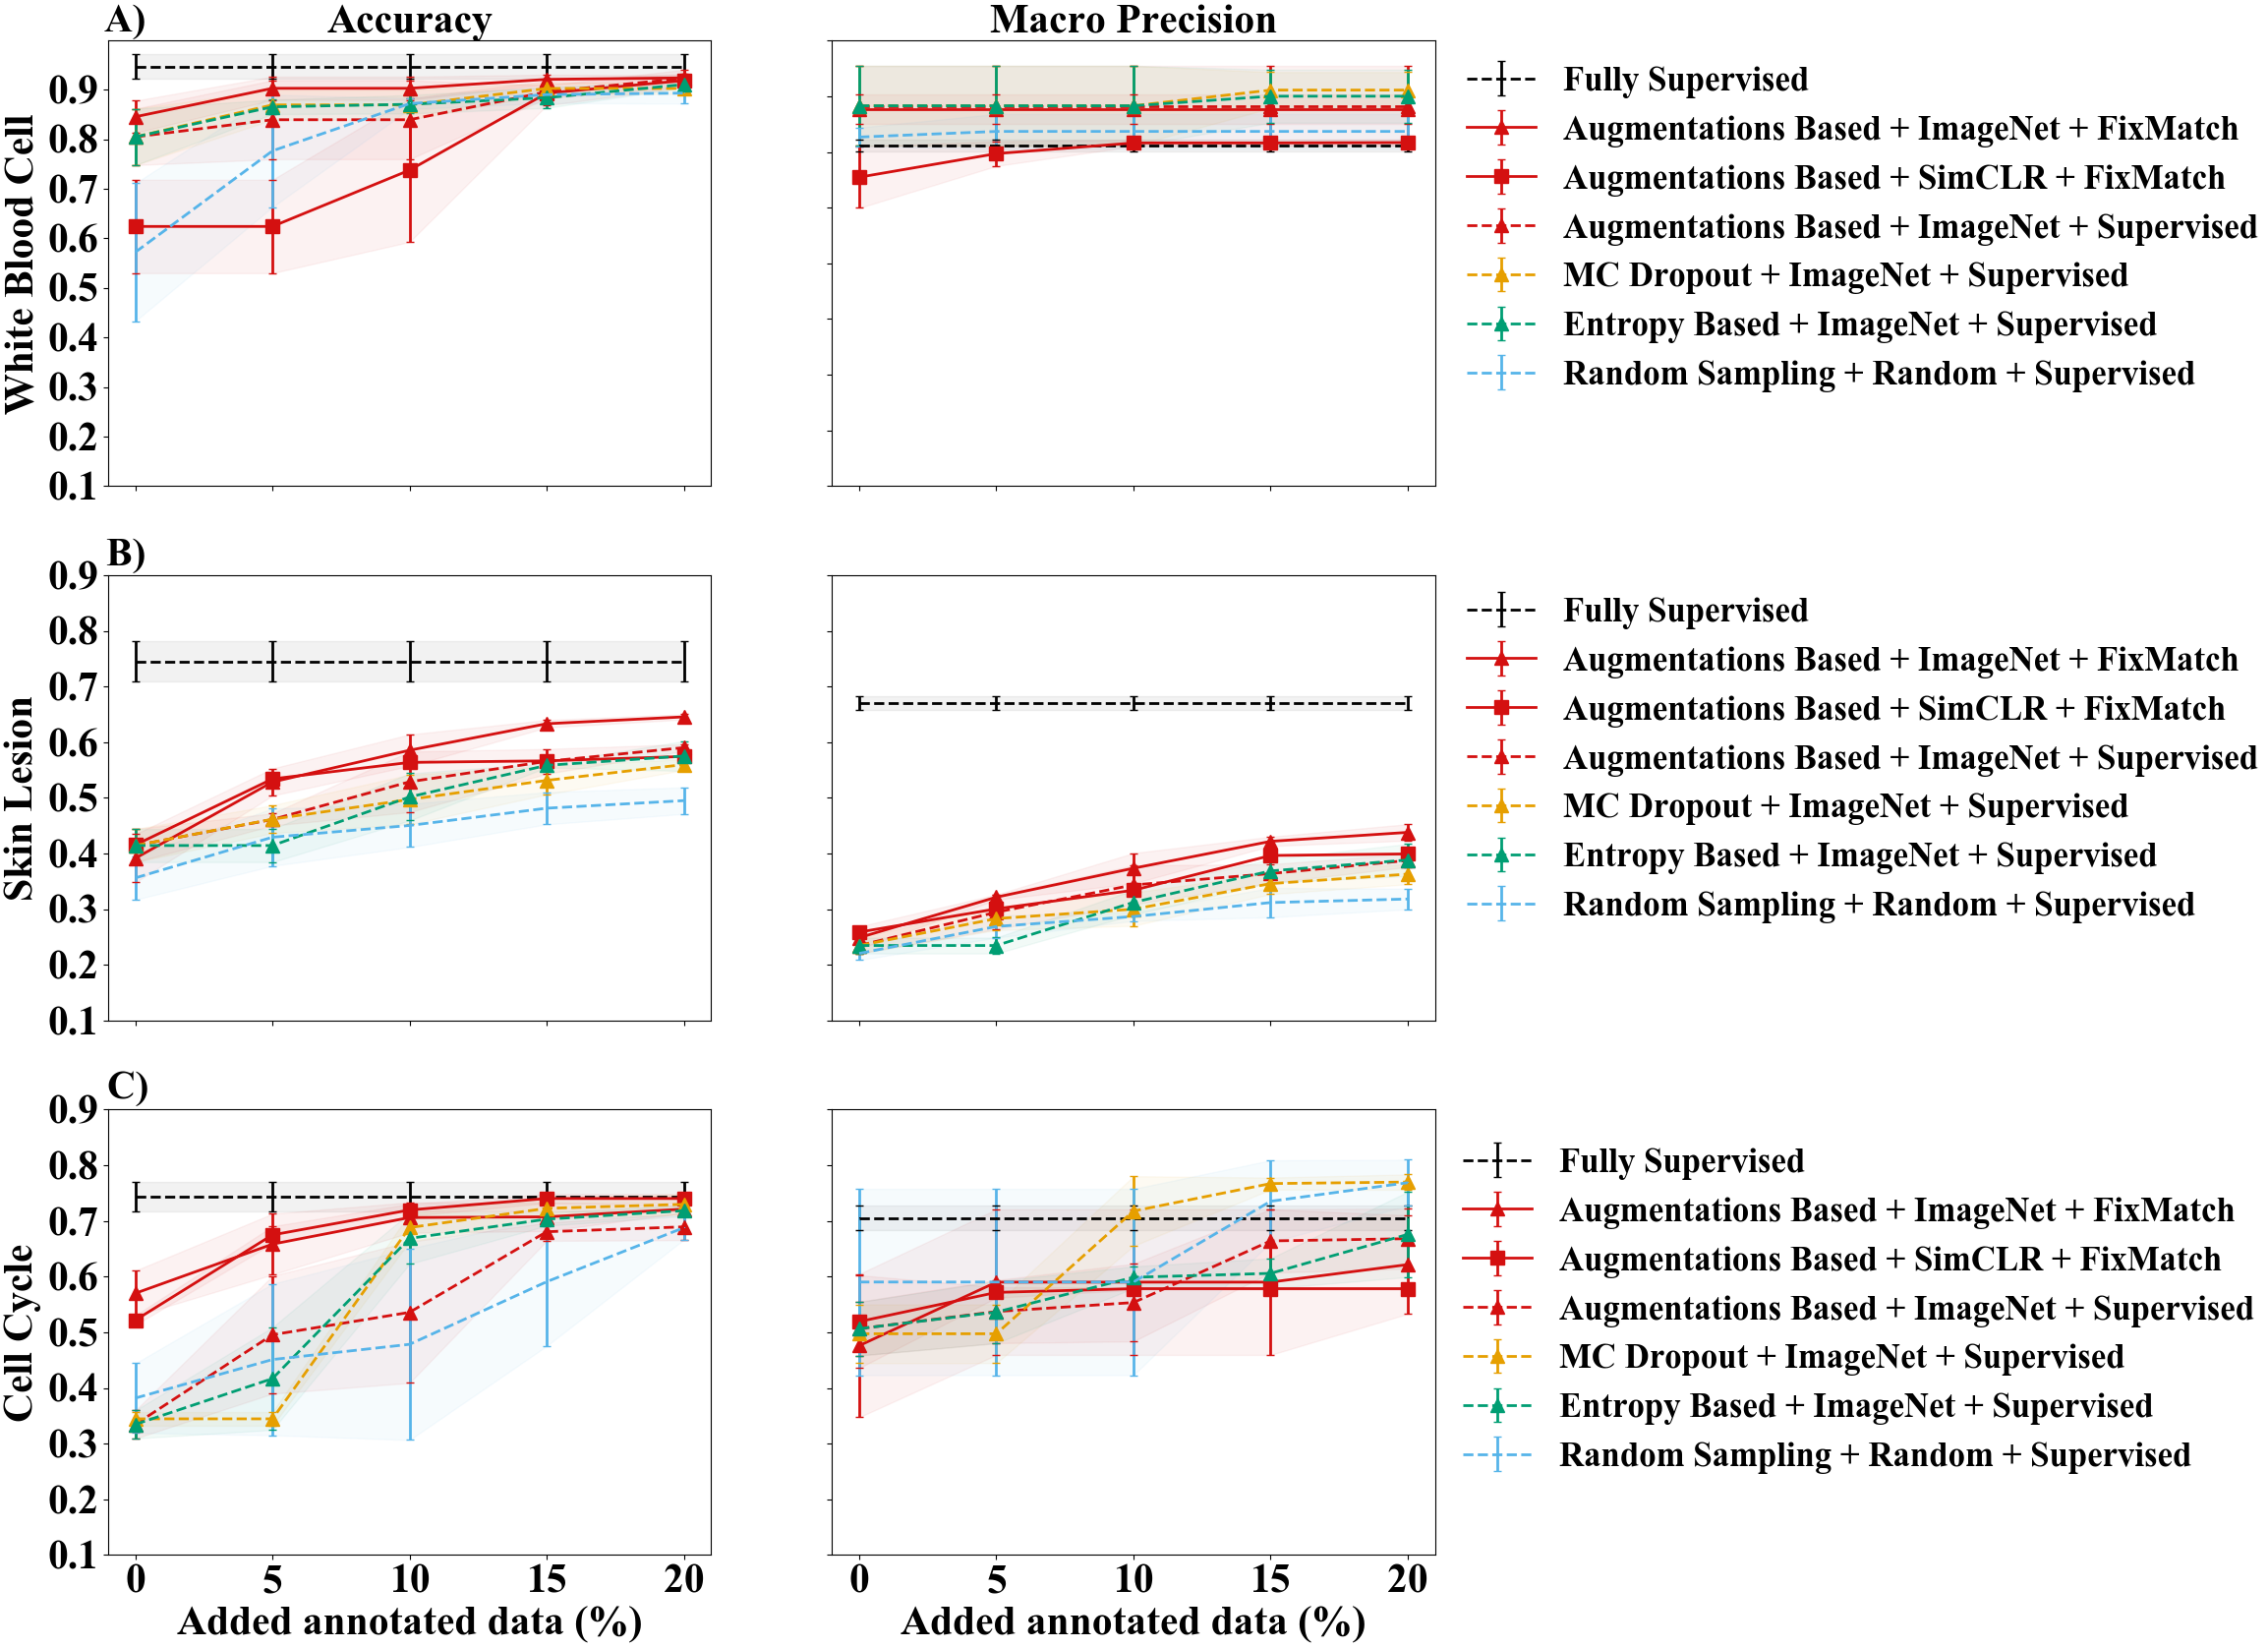
\includegraphics[width=\textwidth]{figures/fig_3_acc_precision.png}
\caption{The combination of augmentation-based sampling, SimCLR or ImageNet pre-training and semi-supervised training with FixMatch is the optimal strategy on all three biomedical datasets. Mean $\pm$ standard deviation of the macro recall are shown after 4-fold cross-validation. (A) On the white blood cell dataset the optimal strategy with ImageNet initialization outperformed all other baseline methods for each active learning iteration by at least 3\%. With only 20\% of added annotated data, this combination performs almost as good as a fully supervised trained model. (B) On the skin lesion dataset the optimal strategies with ImageNet and SimCLR pre-training outperformed all other methods. During the initial step (no added data) and 5\% added data (first iteration), both optimal strategies were at least 4\% better than all baseline methods. (C) On the cell cycle dataset the optimal strategies with ImageNet and SimCLR pre-training were ~14\% better than all baseline methods with no added data. Nonetheless, the optimal strategy with ImageNet pre-training did not improve as rapidly as the optimal strategy with SimCLR pre-training. The optimal strategy with SimCLR pre-training was ~3\% better than all baseline methods and only 6\% worse than the fully supervised trained model, however using only 20\% of annotated data.}
\label{fig:all_acc_precision}
\end{figure}

\begin{figure}[htbp]
\centering
\captionsetup{format=plain}
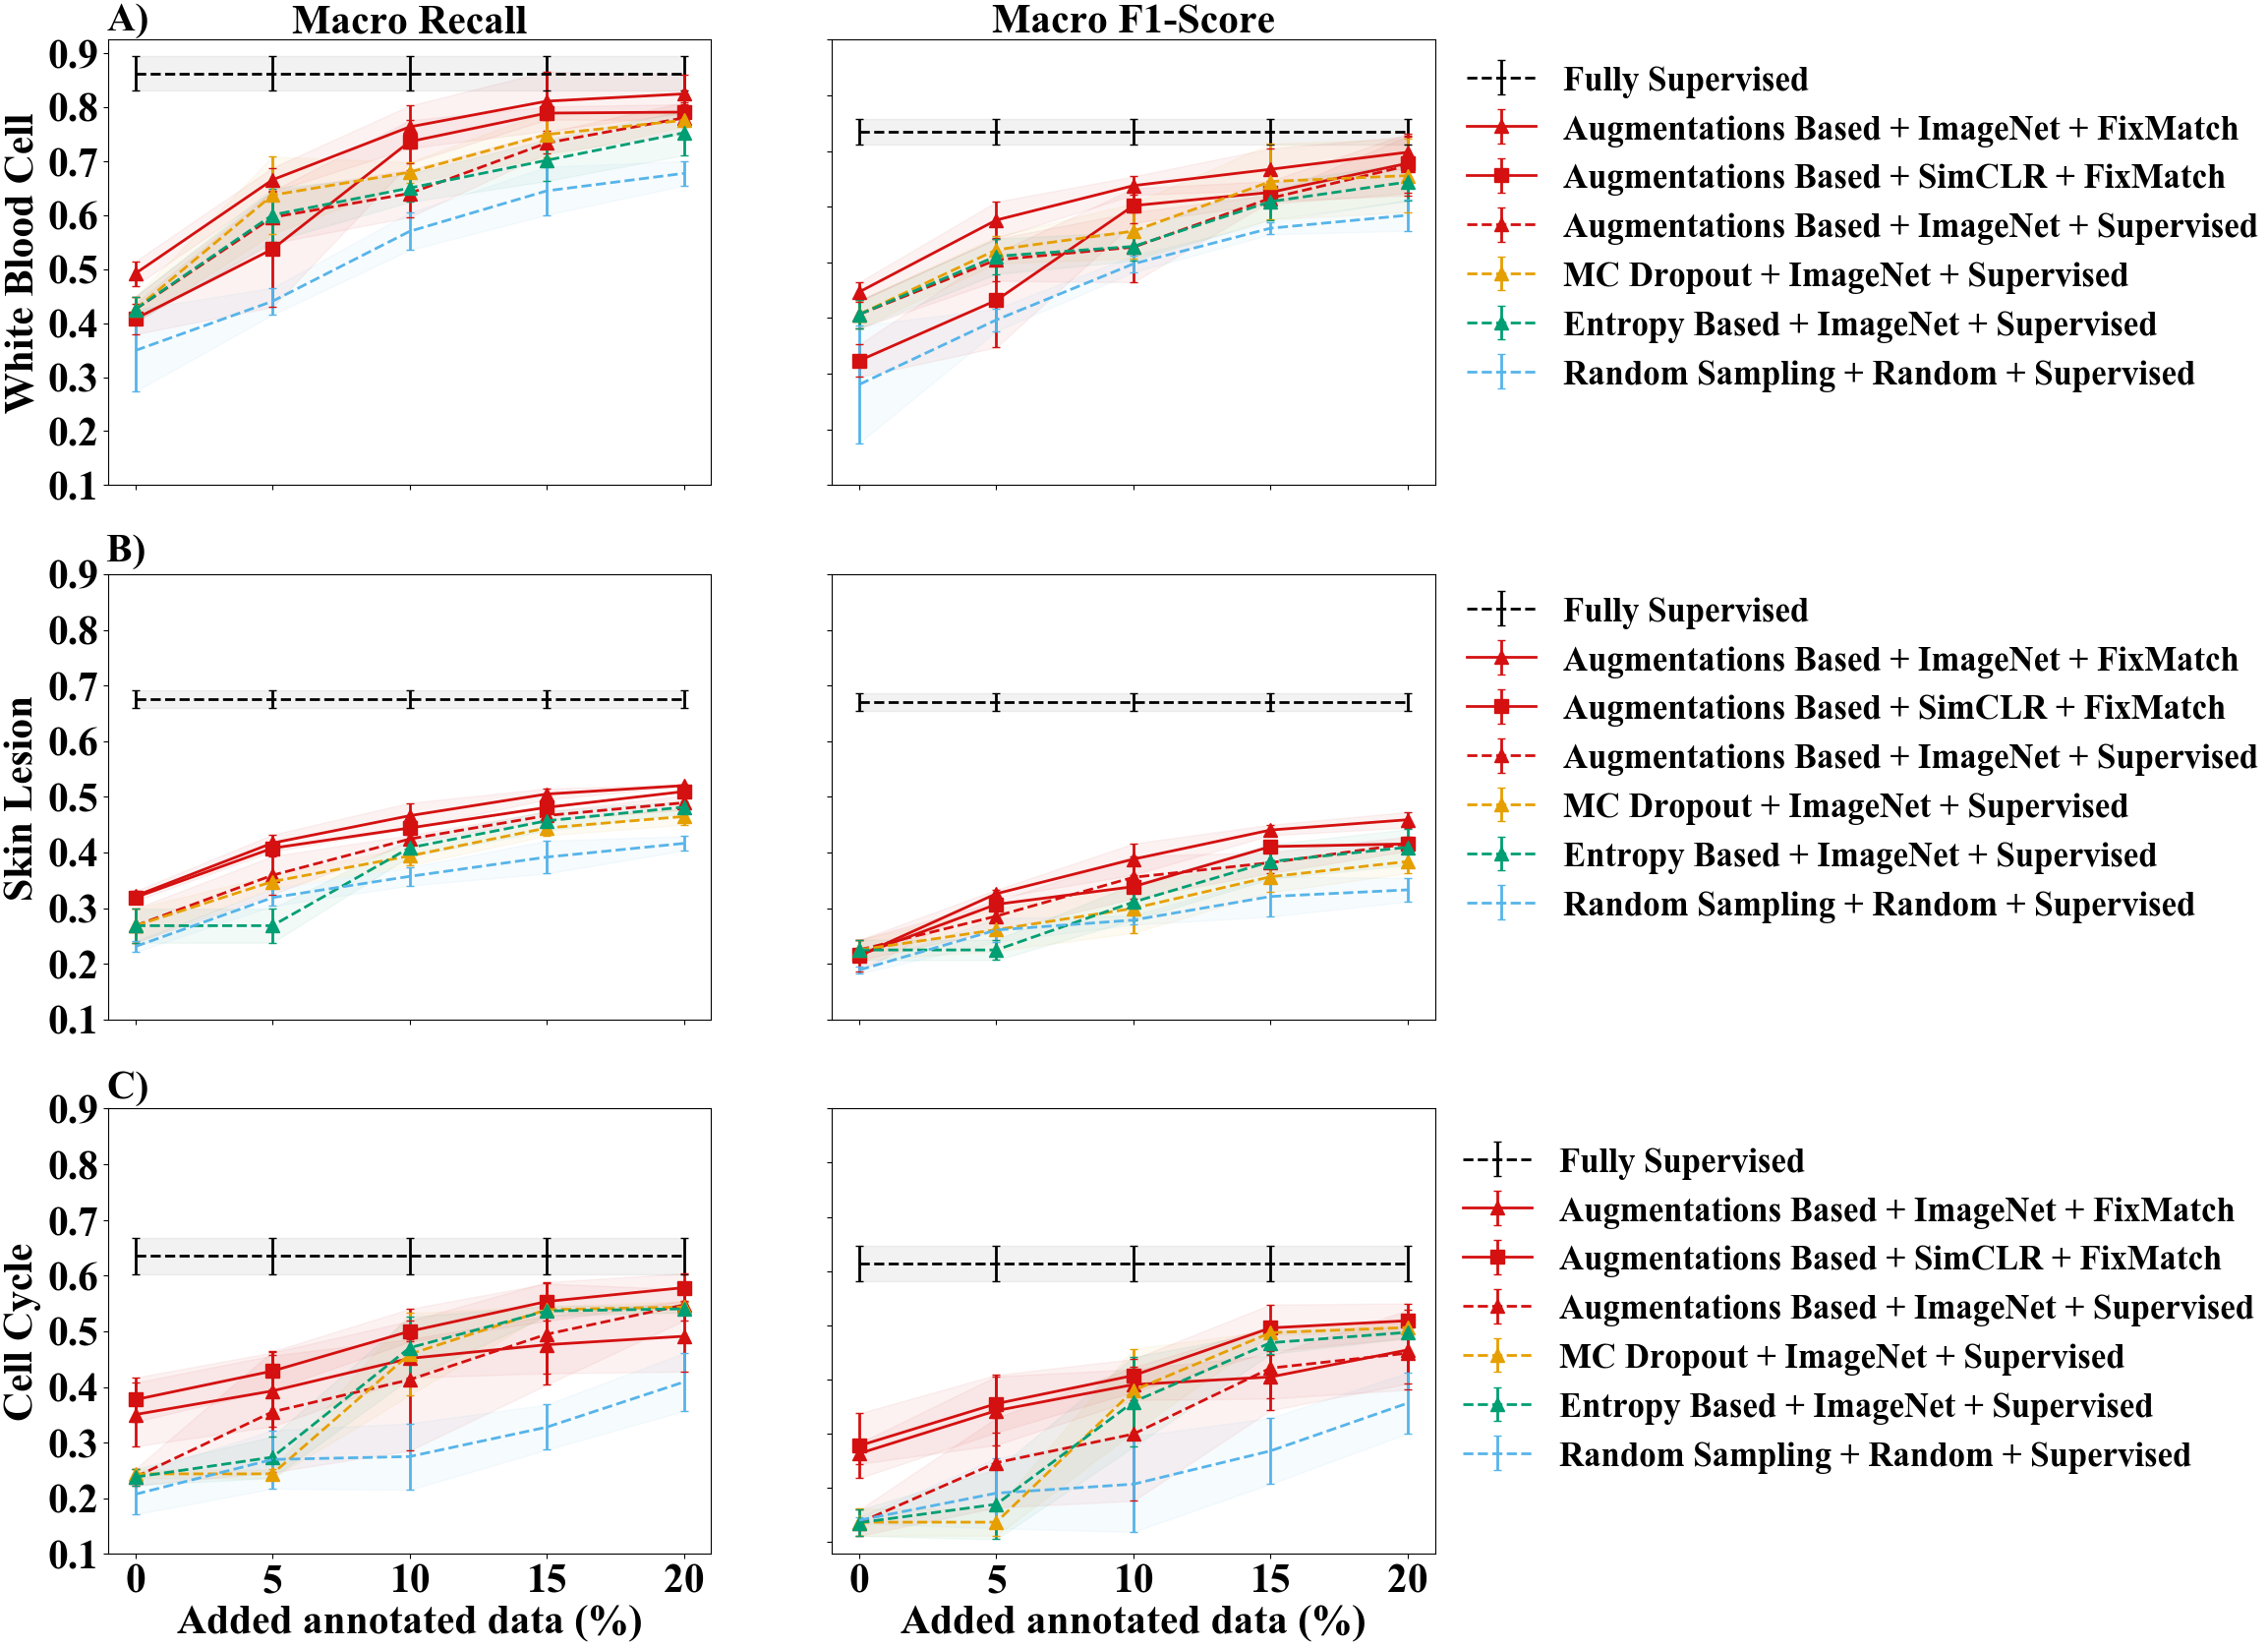
\includegraphics[width=\textwidth]{figures/fig_3_recall_f1.png}
\caption{The combination of augmentation-based sampling, SimCLR or ImageNet pre-training and semi-supervised training with FixMatch is the optimal strategy on all three biomedical datasets. Mean $\pm$ standard deviation of the macro recall are shown after 4-fold cross-validation. (A) On the white blood cell dataset the optimal strategy with ImageNet initialization outperformed all other baseline methods for each active learning iteration by at least 3\%. With only 20\% of added annotated data, this combination performs almost as good as a fully supervised trained model. (B) On the skin lesion dataset the optimal strategies with ImageNet and SimCLR pre-training outperformed all other methods. During the initial step (no added data) and 5\% added data (first iteration), both optimal strategies were at least 4\% better than all baseline methods. (C) On the cell cycle dataset the optimal strategies with ImageNet and SimCLR pre-training were ~14\% better than all baseline methods with no added data. Nonetheless, the optimal strategy with ImageNet pre-training did not improve as rapidly as the optimal strategy with SimCLR pre-training. The optimal strategy with SimCLR pre-training was ~3\% better than all baseline methods and only 6\% worse than the fully supervised trained model, however using only 20\% of annotated data.}
\label{fig:all_recall_f1}
\end{figure}

\newpage

\section{Recommended strategy}
As a result of the previous sections, the optimal strategy is identified as the combination of augmentation-based sampling, ImageNet/SimCLR pre-training and FixMatch to show the best results on 3 biomedical datasets. As illustrated in Figure 3, the ImageNet pre-training works better for white blood cells and the skin lesions from the initial step. SimCLR pre-training seems to work best on the cell cycle data. Therefore, the recommended strategy is to find the best pre-training method on the initial step and combine it with augmentation-based sampling and FixMatch during training. The results of the recommended strategy improves macro recall by 4\% for white blood cells data, 3\% on skin lesions data and 3\% for cell cycle data on the last iteration, with respect to the best conventional active learning method for each dataset.

% Change this figure into a table and also change the table caption
\begin{figure}[htbp]
\centering
\captionsetup{format=plain}
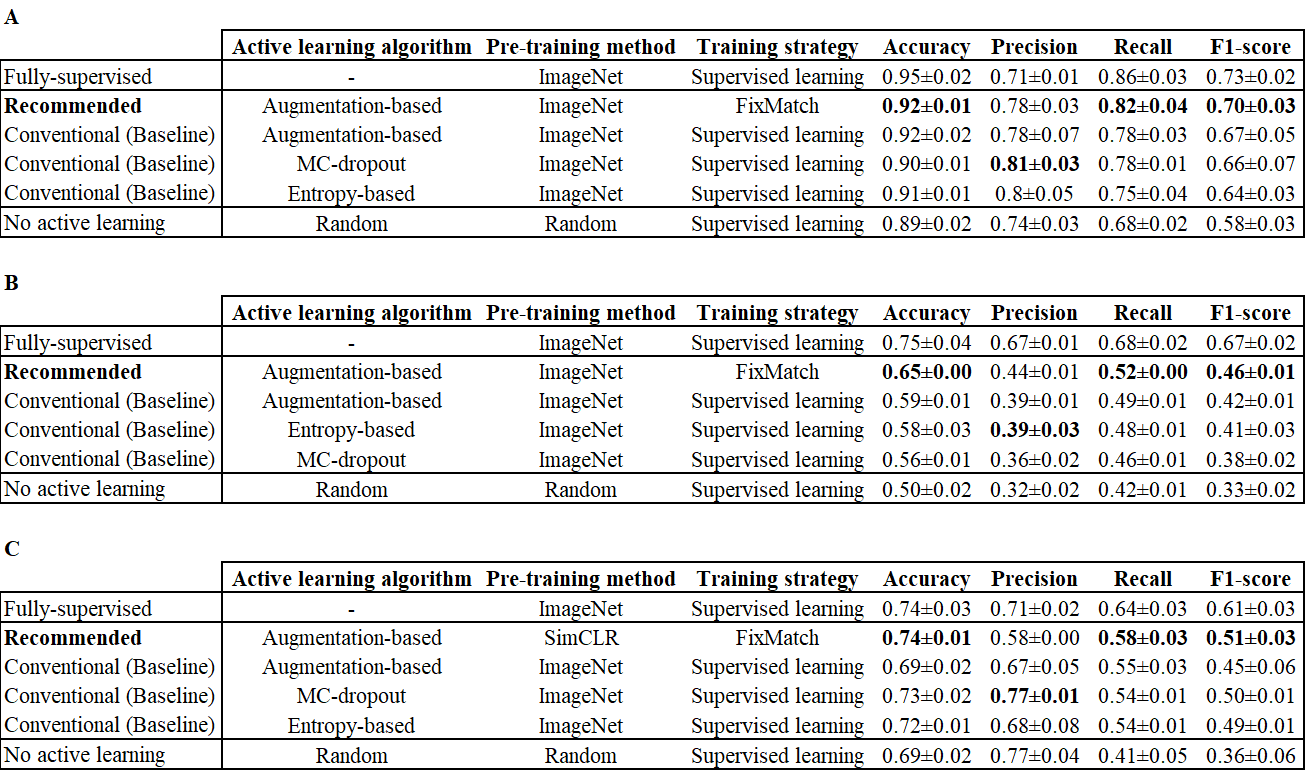
\includegraphics[width=\textwidth]{figures/fig_results_3.png}
\caption{Comparing the results of the last iteration, the recommended strategies outperform conventional annotation-efficient learning. (A) On the white blood cell dataset, the combination of augmentation-based sampling, ImageNet pretraining and FixMatch training brings an improvement of 4\% on macro recall and 3\% on F1-score over the highest baseline. With using only 20\% of added labeled data, this strategy is only 4\% lower in recall and 3\% lower with respect to the F1-score as compared to fully-supervised training. (B) On the skin lesions dataset, the recommended strategy brings an improvement of 3\% on macro recall, 5\% improvement on precision and 6\% on F1-score. The high recall difference to the fully-supervised results shows that the amount of labeled data was not enough and more iterations were needed. (C) On the cell cycle dataset, the recommended strategy brings an improvement of 3\% on recall and 6\% on F1-score.
}
\label{fig:results_3}
\end{figure}
% !TeX root = ../main.tex
% Add the above to each chapter to make compiling the PDF easier in some editors.

\chapter{Conclusion}\label{chapter:conclusion}

In this paper, we have investigated the performance of different annotation-efficient learning strategies for biomedical image classification. First, we showed that for classifying white blood cells into 10 different classes, active learning can boost macro recall. Second, we showed using ImageNet and SimCLR pre-training can increase the performance further. However, their contribution is dataset dependent: While for white blood cell and skin lesion dataset, ImageNet weight led to better performance, SimCLR performed better for classifying cell cycles (Figure 3). This might be due to the nature of images: Cell cycle data is captured by fluorescent imaging which follows a very different color distribution than other technologies such as dermoscopy cameras, which are closer to natural images. Therefore, ImageNet pre-training might not be the preferred way for such data.
We also showed that by incorporating unlabeled data in the training process in a semi-supervised manner, one can improve the performance of the classification noticeably. Finally, by doing a grid-search over all the possible algorithms and strategies (Table 1), we found out that the combination of ImageNet or SimCLR pre-training, FixMatch semi-supervised learning and augmentation-based sampling can improve existing methods for every dataset. The reason for this is probably the fact that while training FixMatch, the network faces many different augmentations for each image and learns to make a robust prediction. Augmentation-based sampling relies on the same idea for finding those images where predictions were not robust enough. 

As a result of this study, we propose an annotation-efficient strategy for biomedical imaging active learning tasks where unlabeled data is abundant (Figure 4). We split our strategy into two parts including pre-training and active learning. First, we suggest to pre-train the network using SimCLR. Then compare FixMatch initialized with ImageNet weights to SimCLR pre-training. By comparing the results, select the best pre-training method. Eventually for the active learning part, we recommend to train FixMatch along with the best pre-training method and augmentation-based sampling to obtain optimal results.

Although our work shows potential for improvement of annotation-efficient learning for three biomedical image classification datasets, the methodology should be tested on more datasets to gain insights into correlations between dataset characteristics and the performance of the applied methods. Due to the computational costs we used a fixed architecture and a fixed set of parameters. As the next step, we will try different architectures and parameters and evaluate the results accordingly. Also, a variety of active learning, semi-supervised and self-supervised learning methods should be added to the work to find the optimal strategy. Finally, to make our findings relevant to the biomedical deep learning field, implementations of the combined methods that allow for quick and easy application need to be provided in an open source implementation.

\begin{figure}[htbp]
\centering
\captionsetup{format=plain}
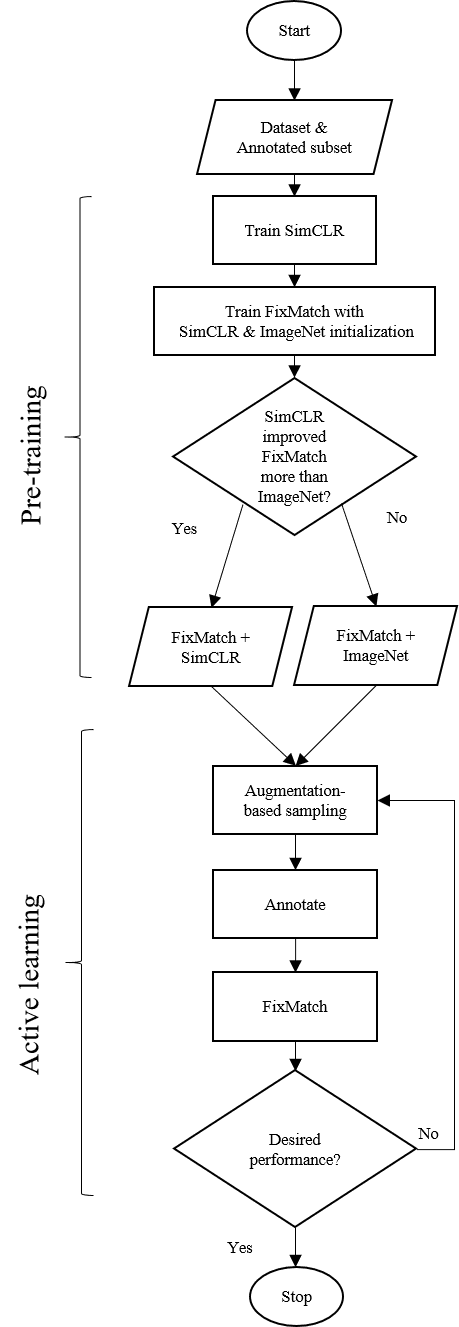
\includegraphics[height=0.65\textheight]{figures/fig_results_4.png}
\caption{Recommended strategy for annotation-efficient classification of biomedical image data involves SimCLR or ImageNet pre-training, FixMatch as the semi-supervised algorithm for training and augmentation-based sampling during active learning until the desired performance is reached.}
\label{fig:results_4}
\end{figure}

\appendix{}

\microtypesetup{protrusion=false}
\listoffigures{}
\listoftables{}
\microtypesetup{protrusion=true}
\printbibliography{}

\end{document}
